\documentclass[11pt]{article}

\usepackage[utf8]{inputenc}
\usepackage[T1]{fontenc}
\usepackage{mathptmx}
\usepackage[scaled=0.92]{helvet}
\usepackage{courier}
\usepackage[margin=1in]{geometry}
\usepackage{microtype}
\usepackage{amsmath,amssymb}
\usepackage{booktabs}
\usepackage{graphicx}
\usepackage{xcolor}
\usepackage{enumitem}
\usepackage{caption}
\usepackage[round,sort&compress]{natbib}
\usepackage[colorlinks=true,linkcolor=blue!55!black,citecolor=blue!55!black,urlcolor=blue!55!black]{hyperref}
\hypersetup{pdftitle={Know Less, Read More: Toward a Minimal Base Curriculum for Small In-Context Learners},pdfauthor={Davitotty1}}

\captionsetup{font=small,labelfont=bf}
\renewcommand{\topfraction}{0.9}
\renewcommand{\bottomfraction}{0.8}
\renewcommand{\textfraction}{0.08}
\renewcommand{\floatpagefraction}{0.85}
\setlist{itemsep=2pt,topsep=4pt}
\newcommand{\tok}[1]{\texttt{#1}}
\newcommand{\skill}[1]{\textsc{#1}}

% ---------------------------------------------------------------------------
% Numbers and tables below are generated by make_results.py from the JSON logs
% of the runs; nothing in gen/ is typed by hand.
% ---------------------------------------------------------------------------
\newcommand{\EFourMaxSeeds}{3}
\newcommand{\EFourMinSeeds}{3}
\newcommand{\EFourTrainMapsFirst}{1{,}500, 2{,}000, 2{,}500}
\newcommand{\EFourTrainMapsFollowMap}{100.0}
\newcommand{\EFourTrainMapsFollowMapList}{100.0, 100.0 and 100.0}
\newcommand{\EFourTrainMapsFollowMapMax}{100.0}
\newcommand{\EFourTrainMapsFollowMapMin}{100.0}
\newcommand{\EFourTrainMapsFollowMapSolved}{3}
\newcommand{\EFourTrainMapsFollowPerm}{100.0}
\newcommand{\EFourTrainMapsFollowPermList}{100.0, 100.0 and 100.0}
\newcommand{\EFourTrainMapsFollowPermMax}{100.0}
\newcommand{\EFourTrainMapsFollowPermMin}{100.0}
\newcommand{\EFourTrainMapsFollowPermSolved}{3}
\newcommand{\EFourTrainMapsSeeds}{3}
\newcommand{\EFourTrainPermsFirst}{never, never, never}
\newcommand{\EFourTrainPermsFollowMap}{31.6}
\newcommand{\EFourTrainPermsFollowMapList}{27.0, 42.1 and 25.8}
\newcommand{\EFourTrainPermsFollowMapMax}{42.1}
\newcommand{\EFourTrainPermsFollowMapMin}{25.8}
\newcommand{\EFourTrainPermsFollowMapSolved}{0}
\newcommand{\EFourTrainPermsFollowPerm}{38.7}
\newcommand{\EFourTrainPermsFollowPermList}{30.3, 52.5 and 33.3}
\newcommand{\EFourTrainPermsFollowPermMax}{52.5}
\newcommand{\EFourTrainPermsFollowPermMin}{30.3}
\newcommand{\EFourTrainPermsFollowPermSolved}{0}
\newcommand{\EFourTrainPermsSeeds}{3}
\newcommand{\EOneMFourNewComposeTwo}{21.2}
\newcommand{\EOneMFourNewComposeTwoList}{21.2}
\newcommand{\EOneMFourNewComposeTwoMax}{21.2}
\newcommand{\EOneMFourNewComposeTwoMin}{21.2}
\newcommand{\EOneMFourNewComposeTwoSolved}{0}
\newcommand{\EOneMFourNewFollow}{22.8}
\newcommand{\EOneMFourNewFollowList}{22.8}
\newcommand{\EOneMFourNewFollowMax}{22.8}
\newcommand{\EOneMFourNewFollowMin}{22.8}
\newcommand{\EOneMFourNewFollowSolved}{0}
\newcommand{\EOneMFourSeeds}{1}
\newcommand{\EOneMFourSeenComposeTwo}{100.0}
\newcommand{\EOneMFourSeenComposeTwoList}{100.0}
\newcommand{\EOneMFourSeenComposeTwoMax}{100.0}
\newcommand{\EOneMFourSeenComposeTwoMin}{100.0}
\newcommand{\EOneMFourSeenComposeTwoSolved}{1}
\newcommand{\EOneMFourSeenFollow}{100.0}
\newcommand{\EOneMFourSeenFollowList}{100.0}
\newcommand{\EOneMFourSeenFollowMax}{100.0}
\newcommand{\EOneMFourSeenFollowMin}{100.0}
\newcommand{\EOneMFourSeenFollowSolved}{1}
\newcommand{\EOneMInfNewComposeTwo}{100.0}
\newcommand{\EOneMInfNewComposeTwoList}{100.0 and 100.0}
\newcommand{\EOneMInfNewComposeTwoMax}{100.0}
\newcommand{\EOneMInfNewComposeTwoMin}{100.0}
\newcommand{\EOneMInfNewComposeTwoSolved}{2}
\newcommand{\EOneMInfNewFollow}{100.0}
\newcommand{\EOneMInfNewFollowList}{100.0 and 100.0}
\newcommand{\EOneMInfNewFollowMax}{100.0}
\newcommand{\EOneMInfNewFollowMin}{100.0}
\newcommand{\EOneMInfNewFollowSolved}{2}
\newcommand{\EOneMInfSeeds}{2}
\newcommand{\EOneMInfSeenComposeTwo}{100.0}
\newcommand{\EOneMInfSeenComposeTwoList}{100.0 and 100.0}
\newcommand{\EOneMInfSeenComposeTwoMax}{100.0}
\newcommand{\EOneMInfSeenComposeTwoMin}{100.0}
\newcommand{\EOneMInfSeenComposeTwoSolved}{2}
\newcommand{\EOneMInfSeenFollow}{100.0}
\newcommand{\EOneMInfSeenFollowList}{100.0 and 100.0}
\newcommand{\EOneMInfSeenFollowMax}{100.0}
\newcommand{\EOneMInfSeenFollowMin}{100.0}
\newcommand{\EOneMInfSeenFollowSolved}{2}
\newcommand{\EOneMOneNewComposeTwo}{21.3}
\newcommand{\EOneMOneNewComposeTwoList}{21.3}
\newcommand{\EOneMOneNewComposeTwoMax}{21.3}
\newcommand{\EOneMOneNewComposeTwoMin}{21.3}
\newcommand{\EOneMOneNewComposeTwoSolved}{0}
\newcommand{\EOneMOneNewFollow}{20.7}
\newcommand{\EOneMOneNewFollowList}{20.7}
\newcommand{\EOneMOneNewFollowMax}{20.7}
\newcommand{\EOneMOneNewFollowMin}{20.7}
\newcommand{\EOneMOneNewFollowSolved}{0}
\newcommand{\EOneMOneSeeds}{1}
\newcommand{\EOneMOneSeenComposeTwo}{100.0}
\newcommand{\EOneMOneSeenComposeTwoList}{100.0}
\newcommand{\EOneMOneSeenComposeTwoMax}{100.0}
\newcommand{\EOneMOneSeenComposeTwoMin}{100.0}
\newcommand{\EOneMOneSeenComposeTwoSolved}{1}
\newcommand{\EOneMOneSeenFollow}{100.0}
\newcommand{\EOneMOneSeenFollowList}{100.0}
\newcommand{\EOneMOneSeenFollowMax}{100.0}
\newcommand{\EOneMOneSeenFollowMin}{100.0}
\newcommand{\EOneMOneSeenFollowSolved}{1}
\newcommand{\EOneMOneSixNewComposeTwo}{21.1}
\newcommand{\EOneMOneSixNewComposeTwoList}{21.1}
\newcommand{\EOneMOneSixNewComposeTwoMax}{21.1}
\newcommand{\EOneMOneSixNewComposeTwoMin}{21.1}
\newcommand{\EOneMOneSixNewComposeTwoSolved}{0}
\newcommand{\EOneMOneSixNewFollow}{31.4}
\newcommand{\EOneMOneSixNewFollowList}{31.4}
\newcommand{\EOneMOneSixNewFollowMax}{31.4}
\newcommand{\EOneMOneSixNewFollowMin}{31.4}
\newcommand{\EOneMOneSixNewFollowSolved}{0}
\newcommand{\EOneMOneSixSeeds}{1}
\newcommand{\EOneMOneSixSeenComposeTwo}{100.0}
\newcommand{\EOneMOneSixSeenComposeTwoList}{100.0}
\newcommand{\EOneMOneSixSeenComposeTwoMax}{100.0}
\newcommand{\EOneMOneSixSeenComposeTwoMin}{100.0}
\newcommand{\EOneMOneSixSeenComposeTwoSolved}{1}
\newcommand{\EOneMOneSixSeenFollow}{100.0}
\newcommand{\EOneMOneSixSeenFollowList}{100.0}
\newcommand{\EOneMOneSixSeenFollowMax}{100.0}
\newcommand{\EOneMOneSixSeenFollowMin}{100.0}
\newcommand{\EOneMOneSixSeenFollowSolved}{1}
\newcommand{\EOneMSixFourNewComposeTwo}{51.3}
\newcommand{\EOneMSixFourNewComposeTwoList}{74.2 and 28.4}
\newcommand{\EOneMSixFourNewComposeTwoMax}{74.2}
\newcommand{\EOneMSixFourNewComposeTwoMin}{28.4}
\newcommand{\EOneMSixFourNewComposeTwoSolved}{0}
\newcommand{\EOneMSixFourNewFollow}{90.5}
\newcommand{\EOneMSixFourNewFollowList}{100.0 and 81.0}
\newcommand{\EOneMSixFourNewFollowMax}{100.0}
\newcommand{\EOneMSixFourNewFollowMin}{81.0}
\newcommand{\EOneMSixFourNewFollowSolved}{1}
\newcommand{\EOneMSixFourSeeds}{2}
\newcommand{\EOneMSixFourSeenComposeTwo}{99.8}
\newcommand{\EOneMSixFourSeenComposeTwoList}{100.0 and 99.6}
\newcommand{\EOneMSixFourSeenComposeTwoMax}{100.0}
\newcommand{\EOneMSixFourSeenComposeTwoMin}{99.6}
\newcommand{\EOneMSixFourSeenComposeTwoSolved}{2}
\newcommand{\EOneMSixFourSeenFollow}{100.0}
\newcommand{\EOneMSixFourSeenFollowList}{100.0 and 100.0}
\newcommand{\EOneMSixFourSeenFollowMax}{100.0}
\newcommand{\EOneMSixFourSeenFollowMin}{100.0}
\newcommand{\EOneMSixFourSeenFollowSolved}{2}
\newcommand{\EOneMaxSeeds}{2}
\newcommand{\EOneMinSeeds}{1}
\newcommand{\EThreeMaxSeeds}{3}
\newcommand{\EThreeMinSeeds}{1}
\newcommand{\EThreeTiedTwoXOneDepthFive}{21.4}
\newcommand{\EThreeTiedTwoXOneDepthFiveList}{21.4}
\newcommand{\EThreeTiedTwoXOneDepthFiveMax}{21.4}
\newcommand{\EThreeTiedTwoXOneDepthFiveMin}{21.4}
\newcommand{\EThreeTiedTwoXOneDepthFiveSolved}{0}
\newcommand{\EThreeTiedTwoXOneDepthFour}{22.9}
\newcommand{\EThreeTiedTwoXOneDepthFourList}{22.9}
\newcommand{\EThreeTiedTwoXOneDepthFourMax}{22.9}
\newcommand{\EThreeTiedTwoXOneDepthFourMin}{22.9}
\newcommand{\EThreeTiedTwoXOneDepthFourSolved}{0}
\newcommand{\EThreeTiedTwoXOneDepthOne}{100.0}
\newcommand{\EThreeTiedTwoXOneDepthOneList}{100.0}
\newcommand{\EThreeTiedTwoXOneDepthOneMax}{100.0}
\newcommand{\EThreeTiedTwoXOneDepthOneMin}{100.0}
\newcommand{\EThreeTiedTwoXOneDepthOneSolved}{1}
\newcommand{\EThreeTiedTwoXOneDepthSix}{22.1}
\newcommand{\EThreeTiedTwoXOneDepthSixList}{22.1}
\newcommand{\EThreeTiedTwoXOneDepthSixMax}{22.1}
\newcommand{\EThreeTiedTwoXOneDepthSixMin}{22.1}
\newcommand{\EThreeTiedTwoXOneDepthSixSolved}{0}
\newcommand{\EThreeTiedTwoXOneDepthThree}{24.4}
\newcommand{\EThreeTiedTwoXOneDepthThreeList}{24.4}
\newcommand{\EThreeTiedTwoXOneDepthThreeMax}{24.4}
\newcommand{\EThreeTiedTwoXOneDepthThreeMin}{24.4}
\newcommand{\EThreeTiedTwoXOneDepthThreeSolved}{0}
\newcommand{\EThreeTiedTwoXOneDepthTwo}{24.9}
\newcommand{\EThreeTiedTwoXOneDepthTwoList}{24.9}
\newcommand{\EThreeTiedTwoXOneDepthTwoMax}{24.9}
\newcommand{\EThreeTiedTwoXOneDepthTwoMin}{24.9}
\newcommand{\EThreeTiedTwoXOneDepthTwoSolved}{0}
\newcommand{\EThreeTiedTwoXOneParams}{113{,}297}
\newcommand{\EThreeTiedTwoXOneSeeds}{1}
\newcommand{\EThreeTiedTwoXThreeDepthFive}{23.0}
\newcommand{\EThreeTiedTwoXThreeDepthFiveList}{23.0}
\newcommand{\EThreeTiedTwoXThreeDepthFiveMax}{23.0}
\newcommand{\EThreeTiedTwoXThreeDepthFiveMin}{23.0}
\newcommand{\EThreeTiedTwoXThreeDepthFiveSolved}{0}
\newcommand{\EThreeTiedTwoXThreeDepthFour}{23.2}
\newcommand{\EThreeTiedTwoXThreeDepthFourList}{23.2}
\newcommand{\EThreeTiedTwoXThreeDepthFourMax}{23.2}
\newcommand{\EThreeTiedTwoXThreeDepthFourMin}{23.2}
\newcommand{\EThreeTiedTwoXThreeDepthFourSolved}{0}
\newcommand{\EThreeTiedTwoXThreeDepthOne}{100.0}
\newcommand{\EThreeTiedTwoXThreeDepthOneList}{100.0}
\newcommand{\EThreeTiedTwoXThreeDepthOneMax}{100.0}
\newcommand{\EThreeTiedTwoXThreeDepthOneMin}{100.0}
\newcommand{\EThreeTiedTwoXThreeDepthOneSolved}{1}
\newcommand{\EThreeTiedTwoXThreeDepthSix}{22.3}
\newcommand{\EThreeTiedTwoXThreeDepthSixList}{22.3}
\newcommand{\EThreeTiedTwoXThreeDepthSixMax}{22.3}
\newcommand{\EThreeTiedTwoXThreeDepthSixMin}{22.3}
\newcommand{\EThreeTiedTwoXThreeDepthSixSolved}{0}
\newcommand{\EThreeTiedTwoXThreeDepthThree}{46.7}
\newcommand{\EThreeTiedTwoXThreeDepthThreeList}{46.7}
\newcommand{\EThreeTiedTwoXThreeDepthThreeMax}{46.7}
\newcommand{\EThreeTiedTwoXThreeDepthThreeMin}{46.7}
\newcommand{\EThreeTiedTwoXThreeDepthThreeSolved}{0}
\newcommand{\EThreeTiedTwoXThreeDepthTwo}{100.0}
\newcommand{\EThreeTiedTwoXThreeDepthTwoList}{100.0}
\newcommand{\EThreeTiedTwoXThreeDepthTwoMax}{100.0}
\newcommand{\EThreeTiedTwoXThreeDepthTwoMin}{100.0}
\newcommand{\EThreeTiedTwoXThreeDepthTwoSolved}{1}
\newcommand{\EThreeTiedTwoXThreeParams}{113{,}297}
\newcommand{\EThreeTiedTwoXThreeSeeds}{1}
\newcommand{\EThreeTiedTwoXTwoDepthFive}{22.2}
\newcommand{\EThreeTiedTwoXTwoDepthFiveList}{21.5, 21.2 and 23.8}
\newcommand{\EThreeTiedTwoXTwoDepthFiveMax}{23.8}
\newcommand{\EThreeTiedTwoXTwoDepthFiveMin}{21.2}
\newcommand{\EThreeTiedTwoXTwoDepthFiveSolved}{0}
\newcommand{\EThreeTiedTwoXTwoDepthFour}{23.4}
\newcommand{\EThreeTiedTwoXTwoDepthFourList}{22.0, 23.0 and 25.1}
\newcommand{\EThreeTiedTwoXTwoDepthFourMax}{25.1}
\newcommand{\EThreeTiedTwoXTwoDepthFourMin}{22.0}
\newcommand{\EThreeTiedTwoXTwoDepthFourSolved}{0}
\newcommand{\EThreeTiedTwoXTwoDepthOne}{100.0}
\newcommand{\EThreeTiedTwoXTwoDepthOneList}{100.0, 100.0 and 100.0}
\newcommand{\EThreeTiedTwoXTwoDepthOneMax}{100.0}
\newcommand{\EThreeTiedTwoXTwoDepthOneMin}{100.0}
\newcommand{\EThreeTiedTwoXTwoDepthOneSolved}{3}
\newcommand{\EThreeTiedTwoXTwoDepthSix}{21.8}
\newcommand{\EThreeTiedTwoXTwoDepthSixList}{22.6, 21.4 and 21.6}
\newcommand{\EThreeTiedTwoXTwoDepthSixMax}{22.6}
\newcommand{\EThreeTiedTwoXTwoDepthSixMin}{21.4}
\newcommand{\EThreeTiedTwoXTwoDepthSixSolved}{0}
\newcommand{\EThreeTiedTwoXTwoDepthThree}{71.9}
\newcommand{\EThreeTiedTwoXTwoDepthThreeList}{85.6, 100.0 and 30.0}
\newcommand{\EThreeTiedTwoXTwoDepthThreeMax}{100.0}
\newcommand{\EThreeTiedTwoXTwoDepthThreeMin}{30.0}
\newcommand{\EThreeTiedTwoXTwoDepthThreeSolved}{1}
\newcommand{\EThreeTiedTwoXTwoDepthTwo}{100.0}
\newcommand{\EThreeTiedTwoXTwoDepthTwoList}{100.0, 100.0 and 100.0}
\newcommand{\EThreeTiedTwoXTwoDepthTwoMax}{100.0}
\newcommand{\EThreeTiedTwoXTwoDepthTwoMin}{100.0}
\newcommand{\EThreeTiedTwoXTwoDepthTwoSolved}{3}
\newcommand{\EThreeTiedTwoXTwoParams}{113{,}297}
\newcommand{\EThreeTiedTwoXTwoSeeds}{3}
\newcommand{\EThreeUntiedFourDepthFive}{21.6}
\newcommand{\EThreeUntiedFourDepthFiveList}{20.6, 21.8 and 22.4}
\newcommand{\EThreeUntiedFourDepthFiveMax}{22.4}
\newcommand{\EThreeUntiedFourDepthFiveMin}{20.6}
\newcommand{\EThreeUntiedFourDepthFiveSolved}{0}
\newcommand{\EThreeUntiedFourDepthFour}{31.3}
\newcommand{\EThreeUntiedFourDepthFourList}{22.7, 48.1 and 23.1}
\newcommand{\EThreeUntiedFourDepthFourMax}{48.1}
\newcommand{\EThreeUntiedFourDepthFourMin}{22.7}
\newcommand{\EThreeUntiedFourDepthFourSolved}{0}
\newcommand{\EThreeUntiedFourDepthOne}{100.0}
\newcommand{\EThreeUntiedFourDepthOneList}{100.0, 100.0 and 100.0}
\newcommand{\EThreeUntiedFourDepthOneMax}{100.0}
\newcommand{\EThreeUntiedFourDepthOneMin}{100.0}
\newcommand{\EThreeUntiedFourDepthOneSolved}{3}
\newcommand{\EThreeUntiedFourDepthSix}{21.8}
\newcommand{\EThreeUntiedFourDepthSixList}{21.2, 23.0 and 21.2}
\newcommand{\EThreeUntiedFourDepthSixMax}{23.0}
\newcommand{\EThreeUntiedFourDepthSixMin}{21.2}
\newcommand{\EThreeUntiedFourDepthSixSolved}{0}
\newcommand{\EThreeUntiedFourDepthThree}{55.0}
\newcommand{\EThreeUntiedFourDepthThreeList}{30.1, 100.0 and 34.9}
\newcommand{\EThreeUntiedFourDepthThreeMax}{100.0}
\newcommand{\EThreeUntiedFourDepthThreeMin}{30.1}
\newcommand{\EThreeUntiedFourDepthThreeSolved}{1}
\newcommand{\EThreeUntiedFourDepthTwo}{89.3}
\newcommand{\EThreeUntiedFourDepthTwoList}{76.4, 100.0 and 91.5}
\newcommand{\EThreeUntiedFourDepthTwoMax}{100.0}
\newcommand{\EThreeUntiedFourDepthTwoMin}{76.4}
\newcommand{\EThreeUntiedFourDepthTwoSolved}{1}
\newcommand{\EThreeUntiedFourParams}{213{,}265}
\newcommand{\EThreeUntiedFourSeeds}{3}
\newcommand{\EThreeUntiedSixDepthFive}{22.1}
\newcommand{\EThreeUntiedSixDepthFiveList}{22.1}
\newcommand{\EThreeUntiedSixDepthFiveMax}{22.1}
\newcommand{\EThreeUntiedSixDepthFiveMin}{22.1}
\newcommand{\EThreeUntiedSixDepthFiveSolved}{0}
\newcommand{\EThreeUntiedSixDepthFour}{25.1}
\newcommand{\EThreeUntiedSixDepthFourList}{25.1}
\newcommand{\EThreeUntiedSixDepthFourMax}{25.1}
\newcommand{\EThreeUntiedSixDepthFourMin}{25.1}
\newcommand{\EThreeUntiedSixDepthFourSolved}{0}
\newcommand{\EThreeUntiedSixDepthOne}{100.0}
\newcommand{\EThreeUntiedSixDepthOneList}{100.0}
\newcommand{\EThreeUntiedSixDepthOneMax}{100.0}
\newcommand{\EThreeUntiedSixDepthOneMin}{100.0}
\newcommand{\EThreeUntiedSixDepthOneSolved}{1}
\newcommand{\EThreeUntiedSixDepthSix}{22.8}
\newcommand{\EThreeUntiedSixDepthSixList}{22.8}
\newcommand{\EThreeUntiedSixDepthSixMax}{22.8}
\newcommand{\EThreeUntiedSixDepthSixMin}{22.8}
\newcommand{\EThreeUntiedSixDepthSixSolved}{0}
\newcommand{\EThreeUntiedSixDepthThree}{65.1}
\newcommand{\EThreeUntiedSixDepthThreeList}{65.1}
\newcommand{\EThreeUntiedSixDepthThreeMax}{65.1}
\newcommand{\EThreeUntiedSixDepthThreeMin}{65.1}
\newcommand{\EThreeUntiedSixDepthThreeSolved}{0}
\newcommand{\EThreeUntiedSixDepthTwo}{95.2}
\newcommand{\EThreeUntiedSixDepthTwoList}{95.2}
\newcommand{\EThreeUntiedSixDepthTwoMax}{95.2}
\newcommand{\EThreeUntiedSixDepthTwoMin}{95.2}
\newcommand{\EThreeUntiedSixDepthTwoSolved}{1}
\newcommand{\EThreeUntiedSixParams}{313{,}233}
\newcommand{\EThreeUntiedSixSeeds}{1}
\newcommand{\ETwoFisherP}{0.030}
\newcommand{\ETwoFullAllSolved}{2}
\newcommand{\ETwoFullComposeThree}{20.5}
\newcommand{\ETwoFullComposeThreeList}{20.2, 20.8, 20.2 and 20.6}
\newcommand{\ETwoFullComposeThreeMax}{20.8}
\newcommand{\ETwoFullComposeThreeMin}{20.2}
\newcommand{\ETwoFullComposeThreeSolved}{0}
\newcommand{\ETwoFullComposeTwo}{74.9}
\newcommand{\ETwoFullComposeTwoList}{100.0, 23.4, 100.0 and 76.3}
\newcommand{\ETwoFullComposeTwoMax}{100.0}
\newcommand{\ETwoFullComposeTwoMin}{23.4}
\newcommand{\ETwoFullComposeTwoSolved}{2}
\newcommand{\ETwoFullFollow}{92.8}
\newcommand{\ETwoFullFollowList}{100.0, 71.2, 100.0 and 99.9}
\newcommand{\ETwoFullFollowMax}{100.0}
\newcommand{\ETwoFullFollowMin}{71.2}
\newcommand{\ETwoFullFollowSolved}{3}
\newcommand{\ETwoFullInduce}{83.7}
\newcommand{\ETwoFullInduceList}{100.0, 35.0, 99.9 and 100.0}
\newcommand{\ETwoFullInduceMax}{100.0}
\newcommand{\ETwoFullInduceMin}{35.0}
\newcommand{\ETwoFullInduceSolved}{3}
\newcommand{\ETwoFullMixedTwo}{25.0}
\newcommand{\ETwoFullMixedTwoList}{25.2, 26.2, 23.2 and 25.3}
\newcommand{\ETwoFullMixedTwoMax}{26.2}
\newcommand{\ETwoFullMixedTwoMin}{23.2}
\newcommand{\ETwoFullMixedTwoSolved}{0}
\newcommand{\ETwoFullSeeds}{4}
\newcommand{\ETwoMaxSeeds}{4}
\newcommand{\ETwoMinSeeds}{4}
\newcommand{\ETwoMixedMax}{26.2}
\newcommand{\ETwoNoComposeComposeThree}{20.5}
\newcommand{\ETwoNoComposeComposeThreeList}{22.3, 20.7, 19.7 and 19.4}
\newcommand{\ETwoNoComposeComposeThreeMax}{22.3}
\newcommand{\ETwoNoComposeComposeThreeMin}{19.4}
\newcommand{\ETwoNoComposeComposeThreeSolved}{0}
\newcommand{\ETwoNoComposeComposeTwo}{19.5}
\newcommand{\ETwoNoComposeComposeTwoList}{17.4, 19.3, 20.6 and 20.8}
\newcommand{\ETwoNoComposeComposeTwoMax}{20.8}
\newcommand{\ETwoNoComposeComposeTwoMin}{17.4}
\newcommand{\ETwoNoComposeComposeTwoSolved}{0}
\newcommand{\ETwoNoComposeFollow}{73.8}
\newcommand{\ETwoNoComposeFollowList}{100.0, 100.0, 20.4 and 74.8}
\newcommand{\ETwoNoComposeFollowMax}{100.0}
\newcommand{\ETwoNoComposeFollowMin}{20.4}
\newcommand{\ETwoNoComposeFollowSolved}{2}
\newcommand{\ETwoNoComposeInduce}{99.8}
\newcommand{\ETwoNoComposeInduceList}{100.0, 100.0, 99.3 and 100.0}
\newcommand{\ETwoNoComposeInduceMax}{100.0}
\newcommand{\ETwoNoComposeInduceMin}{99.3}
\newcommand{\ETwoNoComposeInduceSolved}{4}
\newcommand{\ETwoNoComposeMixedTwo}{20.0}
\newcommand{\ETwoNoComposeMixedTwoList}{16.7, 17.8, 21.8 and 23.8}
\newcommand{\ETwoNoComposeMixedTwoMax}{23.8}
\newcommand{\ETwoNoComposeMixedTwoMin}{16.7}
\newcommand{\ETwoNoComposeMixedTwoSolved}{0}
\newcommand{\ETwoNoComposeSeeds}{4}
\newcommand{\ETwoNoFollowComposeThree}{21.1}
\newcommand{\ETwoNoFollowComposeThreeList}{20.5, 21.4, 21.7 and 20.7}
\newcommand{\ETwoNoFollowComposeThreeMax}{21.7}
\newcommand{\ETwoNoFollowComposeThreeMin}{20.5}
\newcommand{\ETwoNoFollowComposeThreeSolved}{0}
\newcommand{\ETwoNoFollowComposeTwo}{25.3}
\newcommand{\ETwoNoFollowComposeTwoList}{26.4, 25.9, 25.0 and 23.8}
\newcommand{\ETwoNoFollowComposeTwoMax}{26.4}
\newcommand{\ETwoNoFollowComposeTwoMin}{23.8}
\newcommand{\ETwoNoFollowComposeTwoSolved}{0}
\newcommand{\ETwoNoFollowFollow}{19.7}
\newcommand{\ETwoNoFollowFollowList}{19.1, 19.7, 19.4 and 20.8}
\newcommand{\ETwoNoFollowFollowMax}{20.8}
\newcommand{\ETwoNoFollowFollowMin}{19.1}
\newcommand{\ETwoNoFollowFollowSolved}{0}
\newcommand{\ETwoNoFollowInduce}{81.4}
\newcommand{\ETwoNoFollowInduceList}{100.0, 100.0, 91.8 and 34.0}
\newcommand{\ETwoNoFollowInduceMax}{100.0}
\newcommand{\ETwoNoFollowInduceMin}{34.0}
\newcommand{\ETwoNoFollowInduceSolved}{2}
\newcommand{\ETwoNoFollowMixedTwo}{22.0}
\newcommand{\ETwoNoFollowMixedTwoList}{25.1, 25.9, 17.4 and 19.4}
\newcommand{\ETwoNoFollowMixedTwoMax}{25.9}
\newcommand{\ETwoNoFollowMixedTwoMin}{17.4}
\newcommand{\ETwoNoFollowMixedTwoSolved}{0}
\newcommand{\ETwoNoFollowSeeds}{4}
\newcommand{\ETwoNoInduceComposeThree}{20.4}
\newcommand{\ETwoNoInduceComposeThreeList}{19.8, 20.5, 20.3 and 21.1}
\newcommand{\ETwoNoInduceComposeThreeMax}{21.1}
\newcommand{\ETwoNoInduceComposeThreeMin}{19.8}
\newcommand{\ETwoNoInduceComposeThreeSolved}{0}
\newcommand{\ETwoNoInduceComposeTwo}{100.0}
\newcommand{\ETwoNoInduceComposeTwoList}{100.0, 100.0, 100.0 and 100.0}
\newcommand{\ETwoNoInduceComposeTwoMax}{100.0}
\newcommand{\ETwoNoInduceComposeTwoMin}{100.0}
\newcommand{\ETwoNoInduceComposeTwoSolved}{4}
\newcommand{\ETwoNoInduceFollow}{100.0}
\newcommand{\ETwoNoInduceFollowList}{100.0, 100.0, 100.0 and 100.0}
\newcommand{\ETwoNoInduceFollowMax}{100.0}
\newcommand{\ETwoNoInduceFollowMin}{100.0}
\newcommand{\ETwoNoInduceFollowSolved}{4}
\newcommand{\ETwoNoInduceInduce}{20.4}
\newcommand{\ETwoNoInduceInduceList}{20.7, 20.6, 20.6 and 19.5}
\newcommand{\ETwoNoInduceInduceMax}{20.7}
\newcommand{\ETwoNoInduceInduceMin}{19.5}
\newcommand{\ETwoNoInduceInduceSolved}{0}
\newcommand{\ETwoNoInduceMixedTwo}{17.0}
\newcommand{\ETwoNoInduceMixedTwoList}{9.1, 19.0, 20.0 and 20.1}
\newcommand{\ETwoNoInduceMixedTwoMax}{20.1}
\newcommand{\ETwoNoInduceMixedTwoMin}{9.1}
\newcommand{\ETwoNoInduceMixedTwoSolved}{0}
\newcommand{\ETwoNoInduceSeeds}{4}
\newcommand{\ETwoPoolComposeThreeAllRuns}{16}
\newcommand{\ETwoPoolComposeThreeAllSolved}{0}
\newcommand{\ETwoPoolComposeWithFollowRuns}{8}
\newcommand{\ETwoPoolComposeWithFollowSolved}{6}
\newcommand{\ETwoPoolComposeWithoutFollowRuns}{4}
\newcommand{\ETwoPoolComposeWithoutFollowSolved}{0}
\newcommand{\ETwoPoolFollowTrainedRuns}{12}
\newcommand{\ETwoPoolFollowTrainedSolved}{9}
\newcommand{\ETwoPoolInduceTrainedRuns}{12}
\newcommand{\ETwoPoolInduceTrainedSolved}{9}
\newcommand{\ETwoPoolMixedAllRuns}{16}
\newcommand{\ETwoPoolMixedAllSolved}{0}
\newcommand{\ETwoRunsAll}{16}
\newcommand{\GuessFive}{20.9}
\newcommand{\GuessFour}{23.7}
\newcommand{\GuessOne}{20.0}
\newcommand{\GuessSix}{22.4}
\newcommand{\GuessThree}{22.2}
\newcommand{\GuessTwo}{26.7}
\newcommand{\MaxRunMinutes}{23}
\newcommand{\MinRunMinutes}{6}
\newcommand{\NparamsMain}{113{,}297}
\newcommand{\NparamsRounded}{113 thousand}
\newcommand{\TotalCpuHours}{5.4}
\newcommand{\TotalRuns}{38}


\title{\textbf{Know Less, Read More:}\\[2pt]
\Large Toward a Minimal Base Curriculum for Small In-Context Learners}

\author{Davitotty1\\
{\normalsize Independent Researcher}\\
{\normalsize\href{https://github.com/davitotty}{\texttt{github.com/davitotty}}}
}
\date{}

\begin{document}
\maketitle

\begin{abstract}
Small language models are usually judged by how much they know.
We ask how little a model needs to know if the rest can be read from its context.
We frame this as the search for a \emph{base curriculum}: the minimal set of skills that must be in the weights so that task-specific knowledge can be supplied as instructional material at inference time.
We propose a six-layer candidate, a criterion for what belongs in the weights, and a ladder of generalisation that separates memorising a textbook from reading one.
We introduce TinyTextbook, a synthetic benchmark in which each episode is a small textbook of freshly sampled rules followed by exercises, and report a pilot study with transformers of about \NparamsRounded{} parameters trained on a CPU (\TotalRuns{} runs).
Models trained on 16 or fewer distinct textbooks answer perfectly on those and at or near chance on new ones; with enough distinct textbooks they read new ones.
A skill left out of training stays at chance, and without the simplest skill the models did not acquire composition either.
Separately trained skills did not combine: no run exceeded \ETwoMixedMax\% on exercises mixing two of them (guessing: 26.7\%).
Applying the same two layers twice extended the chain of rules a model could follow without adding parameters, but at equal depth looped and unshared models showed no consistent difference.
Outcomes vary between seeds and are reported as counts.
The pilot is small: one to four seeds, one synthetic domain, and a fixed page layout in which values are found by position; retrieval by content was not learned within our budget.
We give a protocol with falsifiable hypotheses for 10--100 million parameters and release the code.

\end{abstract}

% ===========================================================================
\section{Introduction}
% ===========================================================================

A language model with a hundred million parameters has little room for an encyclopedia.
What it might hold instead is the ability to \emph{use} one.
A student who opens a mathematics textbook does not need to have memorised its theorems; she needs to be able to read a definition, follow a worked example, apply a stated rule to a new case, chain two rules together, and notice when an answer does not check out.
The theorems stay in the book.
This paper asks what the corresponding division of labour looks like for a small transformer: \emph{what is the least that must be stored in the weights so that everything else can be supplied in the context?}

That such a division is possible at all is the lesson of in-context learning (ICL).
Large language models adapt to new tasks from a prompt without any weight update \citep{brown2020gpt3}, and transformers trained from scratch on synthetic data learn to fit whole function classes from in-context examples \citep{garg2022what}, in some cases generalising to datasets that were never part of meta-training \citep{kirsch2022gpicl,hollmann2023tabpfn}.
The ability is itself learned: the weights do not encode the answer, they encode a procedure for extracting the answer from what is in front of the model \citep{akyurek2023what,vonoswald2023gd,bai2023statisticians}.

Two features of this literature leave our question open.
First, the material that is placed in context is almost always a list of $(x, y)$ exemplars drawn from a single function class.
A textbook is a different object: it states rules explicitly, mixes rules with examples, introduces its own notation, and expects the reader to combine several of its statements to answer one exercise.
Second, the question most often asked about pretraining is quantitative: \emph{how many} distinct tasks must be seen before in-context learning emerges \citep{raventos2023diversity,he2024grok,goddard2025when,nguyen2025kinetics}.
The complementary question is qualitative: \emph{which} abilities form the set that has to be in the weights, and which can be left out without loss.
We call that set the \emph{base curriculum}.

Answering the qualitative question matters most for small models.
When capacity is scarce, every fact stored in the weights displaces something else, and a fact that could have been read from the context is the cheapest thing to displace.
If the base curriculum is small and mostly procedural, then a small model that is trained on it and paired with good material could be far more useful than its parameter count suggests.
If instead the base curriculum turns out to be large, or impossible to separate from domain knowledge, that would be an equally useful thing to know.

\paragraph{Contributions.}
\begin{enumerate}
\item \textbf{A formulation} of the problem (Section~\ref{sec:formulation}): open-book learners, a simple admission criterion for what belongs in the weights, and a four-level ladder of generalisation that separates memorising a textbook from reading one.
\item \textbf{A concrete hypothesis} (Section~\ref{sec:curriculum}): a six-layer base curriculum, from parsing notation up to verifying an answer, together with an explicit list of what it excludes.
\item \textbf{TinyTextbook} (Section~\ref{sec:benchmark}): a synthetic benchmark in which every episode is a small textbook followed by exercises, and in which the rules are resampled for every episode so that memorising them is useless. The generator, the model and the training loop fit in one file of about 300 lines, released with this paper.
\item \textbf{A pilot study} (Section~\ref{sec:pilot}) with transformers of roughly \NparamsRounded{} parameters trained on a CPU. Models trained on few distinct textbooks answer perfectly on those and near chance on new ones, while models trained on many read new textbooks; a skill left out of training stays at chance, and leaving out the simplest skill also blocks composition; separately trained skills do not combine without training; and applying the same layers a second time extends the chain of rules a model can follow at no cost in parameters. A fourth experiment shows that a symmetry in the training data can keep the basic reading skill from being learned within the budget, and we report what failed.

\item \textbf{A protocol} (Section~\ref{sec:protocol}) with falsifiable hypotheses for repeating the study at 10--100 million parameters, where the question actually has practical consequences.
\end{enumerate}

\paragraph{Scope.}
The pilot is deliberately tiny, uses one synthetic domain, and covers four of the six proposed layers.
Its role is to show that the question can be posed precisely and measured cheaply, and to report what the first measurements say.
It supports no claim about natural language or about models of practical size; Section~\ref{sec:limitations} lists what would have to be true for the picture to carry over.

% ===========================================================================
\section{Related Work}
% ===========================================================================

\paragraph{In-context learning as a learned algorithm.}
\citet{garg2022what} showed that transformers trained from scratch can learn linear functions, sparse linear functions, decision trees and small neural networks from in-context examples.
Subsequent work characterised the algorithm being implemented, relating it to gradient descent and ridge regression \citep{akyurek2023what,vonoswald2023gd}, to in-context algorithm selection \citep{bai2023statisticians}, and to implicit Bayesian inference \citep{xie2022bayesian}.
At the circuit level, \citet{olsson2022induction} identified induction heads as a mechanism for copying from context.
Prior-data fitted networks apply the same idea to tabular prediction, meta-training on synthetic datasets only \citep{muller2022pfn,hollmann2023tabpfn}.

\paragraph{When does in-context learning emerge?}
\citet{chan2022data} traced the emergence of ICL to distributional properties of the training data and documented a trade-off with in-weights learning; \citet{singh2023transient} found that ICL can emerge and then fade as training continues.
\citet{raventos2023diversity} identified a task-diversity threshold: below it a transformer behaves like a Bayesian estimator whose prior is the finite set of pretraining tasks, and above it the model solves tasks it has never seen.
\citet{kirsch2022gpicl} described transitions between algorithms that generalise, algorithms that memorise, and failure to meta-train, and argued that the accessible state size, more than the parameter count, limits a meta-trained in-context learner.
Related transitions have been reported for modular arithmetic \citep{he2024grok} and analysed in terms of the pretraining task distribution \citep{goddard2025when,letey2025alignment} and of learning dynamics \citep{reddy2023mechanistic,nguyen2025kinetics}.
These studies ask how much diversity is needed; we ask which skills the diverse tasks must exercise.

\paragraph{Meta-training language models to learn in context.}
MetaICL \citep{min2022metaicl} and in-context tuning \citep{chen2022tuning} fine-tune language models on collections of tasks so that they learn new tasks from prompts.
\citet{lake2023mlc} meta-train a transformer on a stream of episodes with changing grammars and obtain systematic compositional generalisation, addressing the failure documented by \citet{lake2018scan}.
Our setting follows the same recipe of episodes with resampled rules, applied to instructional material and organised around the question of which skills are necessary.

\paragraph{Learning from material placed in the context.}
The closest formal treatment is that of \citet{zhu2025context}, who study gradient-based training in which helpful material is present in the context and show, in a simplified setting, an exponential gain in sample efficiency when the model is capable of ICL.
\citet{russin2025interplay} show that in-context and in-weight learning respond differently to the ordering of examples, reproducing curriculum effects known from human learning.
At the system level, retrieval-augmented generation supplies documents to the model at inference time \citep{lewis2020rag}; our question is what the model reading those documents must already be able to do, and \citet{liu2023lost} show that the reading itself is not robust: performance drops when the relevant information sits in the middle of a long context.

\paragraph{Small models and curricula.}
Restricting and curating the training distribution lets very small models acquire abilities usually associated with larger ones, for instance coherent text \citep{eldan2023tinystories}, code \citep{gunasekar2023textbooks} and arithmetic \citep{lee2023arithmetic}.
In that line of work the curated data are absorbed into the weights; here the ``textbook'' stays in the context.
Ordering training from easy to hard is an old idea \citep{elman1993starting,bengio2009curriculum} that has recently been applied to reasoning in small language models \citep{fu2025easy}.

\paragraph{Recurrent depth.}
Composing several rules read from the context is a serial computation, and the depth of a transformer bounds how much of it fits into one forward pass.
Re-applying the same layers is one way to buy depth without parameters.
The idea goes back to Universal Transformers \citep{dehghani2019universal} and adaptive computation time \citep{graves2016act}.
Looped transformers can emulate programmable computers \citep{giannou2023looped}, learn in-context learning algorithms with a fraction of the parameters of an unshared stack \citep{yang2024looped}, and approach the performance of much deeper unshared models on reasoning tasks \citep{saunshi2025latent}.
The approach has been scaled to language-model pretraining \citep{geiping2025recurrent,zhu2025ouro,bae2025mor}, and recursion is central to recent small models for abstract puzzles \citep{wang2025hrm,jolicoeur2025trm}.
Computation carried in hidden states can replace computation written out as a chain of thought \citep{wei2022cot,nye2021scratchpad,hao2025coconut}, which makes it harder to inspect \citep{korbak2025monitorability}; we return to this in Section~\ref{sec:limitations}.

% ===========================================================================
\section{Formulation}
\label{sec:formulation}
% ===========================================================================

\subsection{Open-book learners}

A \emph{task} is a rule set $R$ together with a semantics that assigns to every query $q$ an answer $a = [\![q]\!]_R$.
A \emph{textbook} for $R$ is a token sequence $m$ that specifies $R$, fully or in part; an \emph{exercise} is a pair $(q, a)$.
A \emph{closed-book learner} is a map $q \mapsto \hat a$ and can answer correctly only if $R$ is encoded in its parameters.
An \emph{open-book learner} is a map $(m, q) \mapsto \hat a$.
An ideal open-book learner implements an interpreter: it recovers $R$ from $m$ and evaluates $q$ under it, for every $R$ in some class $\mathcal{R}$ and every faithful rendering $m$ of $R$.

This separates two kinds of knowledge.
\emph{Declarative} knowledge is the content of $R$: it differs from task to task.
\emph{Procedural} knowledge is whatever is needed to implement the interpreter: it is shared by all tasks in $\mathcal{R}$.
The working hypothesis of this paper is that a small model should spend its parameters on the second kind and receive the first kind through $m$.

\subsection{What belongs in the weights}
\label{sec:criterion}

Consider one item of knowledge $z$: a fact, a definition, or a procedure.
We propose that $z$ belongs in the weights if it passes either of two tests.

\begin{description}[leftmargin=1.5em,itemsep=2pt]
\item[Bootstrap.] $z$ is needed to interpret the material itself. The meaning of the notation in which definitions are written cannot be supplied by a definition written in that notation.
\item[Amortisation.] Stating $z$ in the context every time it is needed costs more than storing it once. If $z$ is used in a fraction $\rho_z$ of $N$ deployment queries and takes $c_z$ tokens to state, at a cost $\kappa$ per token, while storing it takes $b_z$ bits of capacity priced at $\lambda$ per bit, then $z$ belongs in the weights when
\begin{equation}
\rho_z \, N \, c_z \, \kappa \;>\; \lambda \, b_z .
\label{eq:amortisation}
\end{equation}
\end{description}

Inequality~\eqref{eq:amortisation} is a framing device and we do not attempt to measure its terms.
Its use is to make two qualitative predictions.
A procedure that almost every query exercises (large $\rho_z$) is worth storing even if it is expensive.
A fact that few queries need (small $\rho_z$) is not, and the smaller the model (the larger $\lambda$), the more facts fall on that side of the line.

\subsection{A ladder of generalisation}
\label{sec:ladder}

High accuracy on exercises does not by itself show that a model reads.
We distinguish four levels, each of which removes one way of succeeding without reading.

\begin{description}[leftmargin=1.5em,itemsep=2pt]
\item[G0: seen textbook, new exercise.] The rules were present in training. A closed-book learner can succeed.
\item[G1: new textbook.] The rules are freshly sampled from the families used in training. Success requires reading the material.
\item[G2: new combination of skills.] The exercise combines trained skills in a way never seen in training, for example a longer chain of rules, or a chain that mixes a stated rule with an induced one.
\item[G3: new family.] The material defines a kind of rule that never occurred in training.
\end{description}

A set of skills is a \emph{sufficient} base curriculum at level G$k$ for a domain if a model trained only on it reaches high accuracy at G$k$, and \emph{minimal} if removing any one skill breaks this.
The pilot in Section~\ref{sec:pilot} measures G0, G1 and G2; G3 is left to the protocol of Section~\ref{sec:protocol}.

% ===========================================================================
\section{The Base-Curriculum Hypothesis}
\label{sec:curriculum}
% ===========================================================================

Table~\ref{tab:curriculum} states the hypothesis.
It is a proposal to be tested, and the tests are leave-one-out ablations: train without one layer, then measure what breaks.

\begin{table}[t]
\centering
\small
\begin{tabular}{@{}llp{6.3cm}l@{}}
\toprule
 & \textbf{Layer} & \textbf{The model can\ldots} & \textbf{Test passed} \\
\midrule
C0 & Parsing        & segment the material into definitions, examples and exercises, and bind names to what they denote & Bootstrap \\
C1 & Primitives     & copy a token, retrieve a value by its key, substitute, compare, count, do small-number arithmetic & Amortisation \\
C2 & Rule following & apply a rule that the material states explicitly & Amortisation \\
C3 & Rule induction & infer a rule that the material only illustrates with examples & Amortisation \\
C4 & Composition    & chain several rules, feeding the output of one into the next & Amortisation \\
C5 & Verification   & check an answer against the rule, and abstain when the material does not determine the answer & Amortisation \\
\bottomrule
\end{tabular}
\caption{The proposed base curriculum. Everything on this list is procedural. The last column gives the test of Section~\ref{sec:criterion} under which the layer is admitted.}
\label{tab:curriculum}
\end{table}

\paragraph{What is excluded.}
Theorems, formulas, constants, named algorithms, and domain procedures such as ``how to solve a quadratic equation'' are left out.
Each is a rule that a textbook can state, so each can travel in the context and be handled by C2 and C4.

\paragraph{Where the line is uncertain.}
Three boundary cases deserve mention, because they are where we expect the hypothesis to be revised.
First, small-number arithmetic is placed in C1 on the grounds that it is used by almost every mathematical rule, but it is declarative in nature and could in principle be supplied as a table; the pilot's induction skill depends on it.
Second, the layers need not be separable in training: an exercise that requires composition necessarily exercises rule following, so ``training without C2'' can only mean removing exercises that consist of rule following alone.
Third, the choice of what counts as one rule family (C3) is a modelling decision that determines how hard G3 is.

% ===========================================================================
\section{TinyTextbook}
\label{sec:benchmark}
% ===========================================================================

TinyTextbook is the smallest setting we could design in which the layers C1--C4 and the levels G0--G2 are all defined.

\paragraph{Episodes.}
Let $\Sigma$ be an alphabet of $K=5$ symbols.
A textbook contains three functions $f_1, f_2, f_3 : \Sigma \to \Sigma$ whose values are fully tabulated, and a fourth function $g$ of which only two input--output examples are shown.
The hidden rule behind $g$ is a cyclic shift, $g(x) = x + s \bmod K$ for a shift $s \in \{1,\dots,K-1\}$ under a fixed ordering of $\Sigma$, so the examples determine it completely, but only for a reader who knows that ordering and can add.
The material is followed by exercises written in prefix notation: \tok{Q $h_d$ $\ldots$ $h_1$ $x$ =} asks for $h_d(\cdots h_1(x))$, and the next token is the answer.
Figure~\ref{fig:episode} shows an example.
All four functions are resampled for every episode.

\begin{figure}[t]
\centering
\fbox{\begin{minipage}{0.93\linewidth}
\small\ttfamily
\textrm{\textbf{Material (19 tokens after the start token)}}\\[2pt]
\hspace*{1em}row of $f_1$:\quad c\ e\ d\ a\ b \hfill\textrm{\emph{i.e.\ $f_1(a){=}c$, $f_1(b){=}e$, $f_1(c){=}d$, \ldots}}\\
\hspace*{1em}row of $f_2$:\quad e\ b\ c\ a\ d\\
\hspace*{1em}row of $f_3$:\quad a\ c\ d\ e\ b\\
\hspace*{1em}examples of $g$:\quad c\ e\quad b\ d \hfill\textrm{\emph{i.e.\ $g(c){=}e$, $g(b){=}d$}}\\[4pt]
\textrm{\textbf{Exercises}}\\[2pt]
\hspace*{1em}\skill{follow}\quad\ \ Q F2 a = \underline{e}\hfill\textrm{\emph{read one entry}}\\
\hspace*{1em}\skill{compose}\quad Q F1 F2 d = \underline{c}\hfill\textrm{\emph{$f_2(d){=}a$, then $f_1(a){=}c$}}\\
\hspace*{1em}\skill{induce}\quad\ \ Q G a = \underline{c}\hfill\textrm{\emph{$g$ shifts by two; $a$ is not among the examples}}\\
\hspace*{1em}\skill{mixed}\quad\ \ \ Q G F3 a = \underline{c}\hfill\textrm{\emph{$f_3(a){=}a$, then $g(a){=}c$; never seen in training}}
\end{minipage}}
\caption{One TinyTextbook episode in the aligned layout. The model is trained to predict only the underlined answers. Every function is resampled for each new episode.}
\label{fig:episode}
\end{figure}

\paragraph{Skills.}
Four kinds of exercise map onto the curriculum.
\skill{follow} asks for one tabulated value and exercises C1 and C2.
\skill{compose} chains $d \ge 2$ tabulated functions and exercises C4.
\skill{induce} queries $g$ on an input that is not among its examples and exercises C3.
\skill{mixed} places $g$ inside a chain of tabulated functions, with the constraint that the input reaching $g$ is not one of its examples; it is never used in training and serves as a G2 test, as do \skill{compose} exercises that are deeper than any seen in training.

\paragraph{Two layouts.}
In the \emph{aligned} layout, used for all results below, the material is a table with a fixed geometry: row $j$ lists $f_j(a), \dots, f_j(e)$ in order, and the function in row $j$ always carries the name token \tok{F}$j$.
A value is found by its address, while what is stored at each address changes with every episode.
The page format is thus in the weights (C0) and the content is in the context.
In the \emph{shuffled} layout each fact is a free-standing triple \tok{name key value}, the triples appear in random order, and the names are redrawn from a pool of eight for every episode, so a value has to be found by matching content.
Section~\ref{sec:negative} reports that the shuffled layout was not learned within our budget.

\paragraph{Training on maps, testing on permutations.}
In training episodes the tabulated functions are arbitrary maps $\Sigma \to \Sigma$; in test episodes they are permutations.
With permutations every symbol appears exactly once in every row, so the answer to a single look-up is uniform over $\Sigma$ unless the entry is read correctly, and the chance level for \skill{follow} is exactly $1/K = 20\%$.
For chains the level is slightly higher, because a function can occur twice in a chain and $f(f(x)) = x$ with probability $2/K$: a guesser that sees the exercise but not the tables reaches \GuessTwo\% at length 2, \GuessThree\% at length 3 and between \GuessFive\% and \GuessFour\% at lengths 4 to 6.
We call these the \emph{guessing levels}; Appendix~\ref{app:details} gives their derivation.
The reason for training on arbitrary maps is empirical and is the subject of experiment E4 (Section~\ref{sec:symmetry}).

\paragraph{Measurement.}
Training episodes contain eight exercises and the loss is the cross-entropy on the eight answer tokens.
Test episodes contain a single exercise placed directly after the material, so that no previously worked exercise can be used as a hint.

% ===========================================================================
\section{Pilot Study}
\label{sec:pilot}
% ===========================================================================

The pilot asks three questions of the smallest models that can answer them.
Does a model trained on textbooks read them or memorise them (E1)?
Which exercise types must be in the training set for which abilities to appear (E2)?
Does re-applying the same layers extend the chain of rules a model can follow (E3)?
A fourth experiment (E4) isolates an effect of the training distribution that we ran into while designing the benchmark.


\paragraph{Setup.}
All models are decoder-only transformers of width 64 with four attention heads.
The default model applies a block of two layers twice, for four layer passes and \NparamsMain{} parameters.
Training takes 5{,}000 steps of 32 episodes (8{,}000 steps in E3) on one CPU core, which is between \MinRunMinutes{} and \MaxRunMinutes{} minutes per run.
Accuracy is measured on 4{,}000 held-out episodes per test, giving a standard error below 0.8 percentage points.
Appendix~\ref{app:details} gives the remaining details, and Appendix~\ref{app:runs} lists every run.
The pilot comprises \TotalRuns{} runs and \TotalCpuHours{} CPU-hours.
The number of seeds per condition is small and is stated with each result; we therefore describe only effects that are large compared with the gap between the guessing level and ceiling.

\subsection{E1: Memorising a textbook versus reading one}

Every training episode draws its textbook from a fixed pool of $M$ textbooks, or from an unlimited supply ($M=\infty$).
The exercises are sampled afresh each time, half of them \skill{follow} and half \skill{compose} at depth 2, and the number of training episodes is the same for every $M$.
We then test on textbooks from the pool (G0) and on new textbooks (G1).

\begin{table}[t]
\centering\small
\begin{tabular}{@{}lcccc@{}}
\toprule
Distinct textbooks & \multicolumn{2}{c}{G0: seen textbooks} & \multicolumn{2}{c}{G1: new textbooks} \\
\cmidrule(lr){2-3}\cmidrule(lr){4-5}
in training ($M$) & \skill{follow} & \skill{compose}-2 & \skill{follow} & \skill{compose}-2 \\
\midrule
1 & 100.0 & 100.0 & 20.7 & 21.3 \\
4 & 100.0 & 100.0 & 22.8 & 21.2 \\
16 & 100.0 & 100.0 & 31.4 & 21.1 \\
64 & 100.0 {\scriptsize\,2/2} & 99.8 {\scriptsize\,2/2} & 90.5 {\scriptsize\,1/2} & 51.3 {\scriptsize\,0/2} \\
$\infty$ & 100.0 {\scriptsize\,2/2} & 100.0 {\scriptsize\,2/2} & 100.0 {\scriptsize\,2/2} & 100.0 {\scriptsize\,2/2} \\
\bottomrule
\end{tabular}

\caption{E1: accuracy (\%) after training on $M$ distinct textbooks. One seed for $M \le 16$; for $M = 64$ and $M = \infty$ the mean of two seeds, followed by the number of seeds that ended at 95\% or above. On new textbooks the guessing level is 20\% for \skill{follow} and \GuessTwo\% for \skill{compose}-2. Seen textbooks tabulate arbitrary maps, as in training; new textbooks tabulate permutations.}
\label{tab:e1}
\end{table}

\begin{figure}[t]
\centering
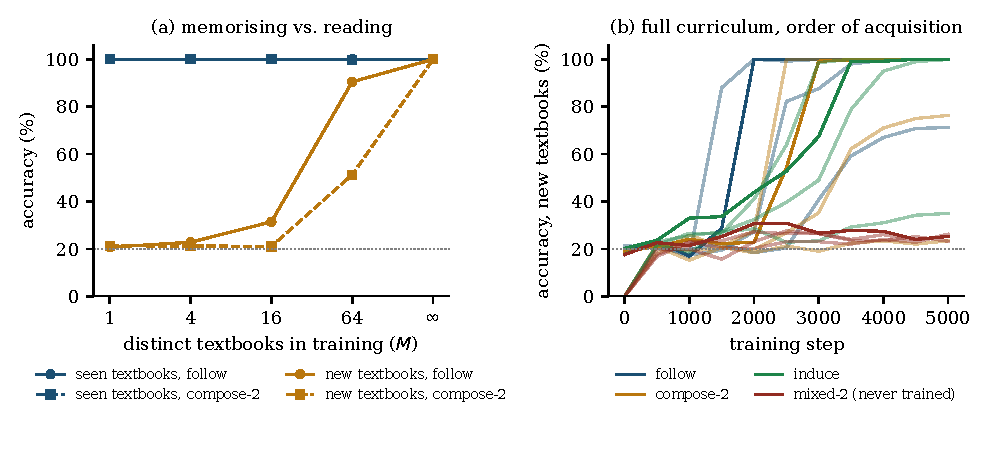
\includegraphics[width=\linewidth]{gen/fig_e1_e2.pdf}
\caption{\textbf{(a)} E1 (means over seeds). All models answer almost perfectly on their training textbooks; only those trained on enough distinct textbooks can use a new one. \textbf{(b)} E2, full curriculum, accuracy on new textbooks during training for each seed (later seeds are drawn lighter). The skills are acquired one after another in abrupt steps, and the never-trained combination \skill{mixed} stays at the guessing level. Dotted line: 20\%.}
\label{fig:e1e2}
\end{figure}

Table~\ref{tab:e1} and Figure~\ref{fig:e1e2}a show the outcome.
Every model answers exercises about its training textbooks almost perfectly.
For $M \le 16$ that is all it can do: on a new textbook, \skill{follow} accuracy is \EOneMOneNewFollow\%, \EOneMFourNewFollow\% and \EOneMOneSixNewFollow\% for $M = 1, 4, 16$.
These models have stored their textbooks in the weights and do not consult the page in front of them.
With $M = 64$ the same architecture, trained for the same number of steps, begins to use textbooks it has never seen: over two seeds it follows their rules at \EOneMSixFourNewFollowList\% and composes them at \EOneMSixFourNewComposeTwoList\%.
With an unlimited supply, both seeds reach at least \EOneMInfNewFollowMin\% on \skill{follow} and \EOneMInfNewComposeTwoMin\% on \skill{compose}.

The switch from memorising to reading as the number of distinct textbooks grows is the instructional-material counterpart of the task-diversity threshold reported for in-context regression \citep{raventos2023diversity} and for modular arithmetic \citep{he2024grok}.
Four points are worth drawing out.

\emph{Accuracy on seen material is uninformative.}
The G0 columns are the same, to within half a point, for models that read and models that do not.
Any evaluation in which the rules were available during training, in whatever form, cannot distinguish the two.

\emph{Variety made the difference, not volume.}
Every model saw the same 160{,}000 training episodes.
What changed is how many different textbooks those episodes were about.
This is the first half of hypothesis H3 in Section~\ref{sec:protocol}.

\emph{The harder skill asks for more variety.}
At $M=64$, \skill{follow} transfers to new textbooks largely or completely (\EOneMSixFourNewFollowList\%) while \skill{compose} lags behind (\EOneMSixFourNewComposeTwoList\%).
With one or two seeds per condition we do not read more into the location of the threshold than that reading begins somewhere between 16 and 64 textbooks for the easier skill and is not complete at 64 for the harder one.

\emph{Knowledge in the weights did not help with a new page.}
The models with $M \le 16$ know their textbooks perfectly and are at or near chance on a new one.
This bears on hypothesis H2 only indirectly: the direct test, adding facts to the weights of a model that already reads, is left to the full-scale study.



\subsection{E2: Which skills have to be trained}

We train four models on new textbooks only ($M=\infty$): one on all three exercise types in equal proportion, and three with one type left out and the remaining two in equal proportion.
\skill{compose} is trained at depth 2 only.
All four are tested on the three trained types and on two G2 tests: \skill{mixed} at depth 2, which combines \skill{compose} with \skill{induce}, and \skill{compose} at depth 3.

\begin{table}[t]
\centering\small
\begin{tabular}{@{}lccccc@{}}
\toprule
& \multicolumn{3}{c}{G1: exercise types in the curriculum} & \multicolumn{2}{c}{G2: never trained} \\
\cmidrule(lr){2-4}\cmidrule(lr){5-6}
Training set & \skill{follow} & \skill{compose}-2 & \skill{induce} & \skill{mixed}-2 & \skill{compose}-3 \\
\midrule
Full curriculum & 92.8 {\scriptsize\,3/4} & 74.9 {\scriptsize\,2/4} & 83.7 {\scriptsize\,3/4} & 25.0 {\scriptsize\,0/4} & 20.5 {\scriptsize\,0/4} \\
without \skill{follow} & 19.7 {\scriptsize\,0/4} & 25.3 {\scriptsize\,0/4} & 81.4 {\scriptsize\,2/4} & 22.0 {\scriptsize\,0/4} & 21.1 {\scriptsize\,0/4} \\
without \skill{compose} & 73.8 {\scriptsize\,2/4} & 19.5 {\scriptsize\,0/4} & 99.8 {\scriptsize\,4/4} & 20.0 {\scriptsize\,0/4} & 20.5 {\scriptsize\,0/4} \\
without \skill{induce} & 100.0 {\scriptsize\,4/4} & 100.0 {\scriptsize\,4/4} & 20.4 {\scriptsize\,0/4} & 17.0 {\scriptsize\,0/4} & 20.4 {\scriptsize\,0/4} \\
\bottomrule
\end{tabular}

\caption{E2: accuracy (\%) on new textbooks after training with one exercise type left out. Each cell gives the mean over seeds, followed by the number of seeds that ended at 95\% or above out of the number run. Guessing levels: 20\% for \skill{follow}, 25\% for \skill{induce}, \GuessTwo\% for \skill{compose}-2, \GuessThree\% for \skill{compose}-3, and 26.7\% on \skill{mixed}-2 for a model that has induced $g$ but cannot combine it with a table look-up (see text).}
\label{tab:e2}
\end{table}

Table~\ref{tab:e2} gives the result, and the first thing it shows is how uneven learning is at this budget.
Skills are acquired in abrupt steps (Figure~\ref{fig:e1e2}b), so a run ends either near ceiling or near chance, and whether a given step arrives before training stops varies with the seed.
Even \skill{follow}, the simplest skill, was solved in only \ETwoPoolFollowTrainedSolved{} of the \ETwoPoolFollowTrainedRuns{} runs whose training set contained it.
Alongside each mean we therefore report how many seeds ended at 95\% or above, and we read the table by comparing those counts.

\paragraph{A skill left out of training was never acquired.}
Without \skill{induce} exercises, \skill{induce} accuracy is at or below its guessing level in every seed (\ETwoNoInduceInduceList\%); without \skill{compose} exercises, so is \skill{compose} (\ETwoNoComposeComposeTwoList\%).
Following and composing do not yield induction, and following and inducing do not yield composition.
Within TinyTextbook each skill is therefore necessary for itself, which is the minimality condition of Section~\ref{sec:ladder} at level G1.

\paragraph{Leaving out the simplest skill removed more than that skill.}
The models trained on \skill{compose} and \skill{induce}, but never on a single look-up, did not learn to look up (\ETwoNoFollowFollowList\% on \skill{follow}) and did not learn to compose either (\ETwoNoFollowComposeTwoList\%, which is the guessing level for two-step chains).
\skill{compose} was solved in \ETwoPoolComposeWithoutFollowSolved{} of \ETwoPoolComposeWithoutFollowRuns{} runs without \skill{follow} in the training set, against \ETwoPoolComposeWithFollowSolved{} of \ETwoPoolComposeWithFollowRuns{} runs with it (the full curriculum and the one without \skill{induce}; one-sided Fisher exact test, $p = \ETwoFisherP$).
A two-step exercise contains two look-ups, so in principle it supervises everything a one-step exercise does.
In practice the one-step exercise acted as a stepping stone without which the two-step skill was not found within the budget.
This also answers, for this benchmark, the worry raised in Section~\ref{sec:curriculum} that rule following cannot be removed separately from composition: it can, and removing it matters.

\paragraph{The full curriculum was not learned in every seed.}
With all three exercise types in training, \ETwoFullFollowSolved{} of \ETwoFullSeeds{} seeds solved \skill{follow}, \ETwoFullComposeTwoSolved{} solved \skill{compose} and \ETwoFullInduceSolved{} solved \skill{induce}; \ETwoFullAllSolved{} solved all three.
\input{sec_pilot_e2_fullseeds.tex}

\paragraph{Trained skills did not combine by themselves.}
\skill{mixed} exercises ask for a tabulated function and the induced function in one chain.
The models trained on the full curriculum score \ETwoFullMixedTwo\% on them (per seed: \ETwoFullMixedTwoList).
This is no better than guessing: when $g$ is the outer function, its input cannot be one of the two example keys, so the answer is one of three symbols that the examples determine, and when $g$ is the inner function the answer is uniform; a model that has induced $g$ and otherwise guesses therefore reaches $(1/3 + 1/5)/2 = 26.7\%$.
None of the \ETwoRunsAll{} runs in this experiment solved \skill{mixed}; the best reached \ETwoMixedMax\%.
Having each skill in the weights was not enough to obtain their combination, which contradicts hypothesis H5 at this scale.
\skill{compose} at depth 3 is likewise at its guessing level in every run, as expected from four layer passes trained on two-step chains; E3 examines depth directly.



\subsection{E3: Recurrent depth}

All models in this experiment are trained on \skill{compose} exercises whose chain length is 1, 2, 3 or 4 with equal probability (length 1 is \skill{follow}), and are tested at lengths 1 to 6.
We compare a block of two layers applied once, twice and three times with unshared stacks of four and six layers.
A looped model with $r$ loops and an unshared model with $2r$ layers perform the same number of layer passes, and the looped one has $1/r$ of the transformer-block parameters.

\begin{table}[t]
\centering\small
\begin{tabular}{@{}lccccccccc@{}}
\toprule
& & Layer & & \multicolumn{4}{c}{G1: chain lengths in training} & \multicolumn{2}{c}{G2: longer} \\
\cmidrule(lr){5-8}\cmidrule(lr){9-10}
Model & Params & passes & Seeds & 1 & 2 & 3 & 4 & 5 & 6 \\
\midrule
2 layers $\times$ 1 loop & 113k & 2 & 1 & 100.0 & 24.9 & 24.4 & 22.9 & 21.4 & 22.1 \\
2 layers $\times$ 2 loops & 113k & 4 & 3 & 100.0 {\scriptsize\,3/3} & 100.0 {\scriptsize\,3/3} & 71.9 {\scriptsize\,1/3} & 23.4 {\scriptsize\,0/3} & 22.2 {\scriptsize\,0/3} & 21.8 {\scriptsize\,0/3} \\
2 layers $\times$ 3 loops & 113k & 6 & 1 & 100.0 & 100.0 & 46.7 & 23.2 & 23.0 & 22.3 \\
4 layers, unshared & 213k & 4 & 3 & 100.0 {\scriptsize\,3/3} & 89.3 {\scriptsize\,1/3} & 55.0 {\scriptsize\,1/3} & 31.3 {\scriptsize\,0/3} & 21.6 {\scriptsize\,0/3} & 21.8 {\scriptsize\,0/3} \\
6 layers, unshared & 313k & 6 & 1 & 100.0 & 95.2 & 65.1 & 25.1 & 22.1 & 22.8 \\
\bottomrule
\end{tabular}

\caption{E3: accuracy (\%) on new textbooks by chain length. Where a model has several seeds, the mean is followed by the number of seeds that ended at 95\% or above out of the number run. Guessing levels for lengths 1 to 6: \GuessOne, \GuessTwo, \GuessThree, \GuessFour, \GuessFive{} and \GuessSix\%.}
\label{tab:e3}
\end{table}

\begin{figure}[t]
\centering
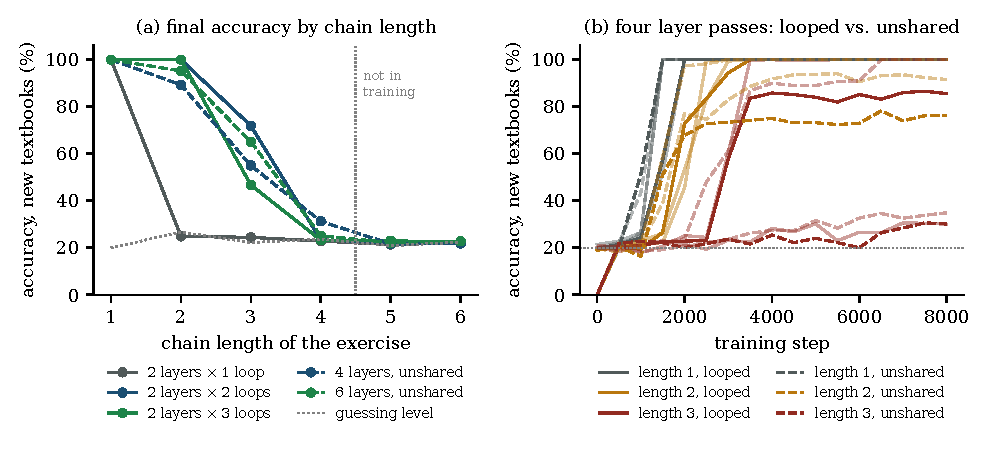
\includegraphics[width=\linewidth]{gen/fig_e3.pdf}
\caption{E3. \textbf{(a)} Final accuracy by chain length, averaged over seeds; solid lines are looped models, dashed lines unshared ones, colour marks the number of layer passes, and the dotted grey curve is the guessing level. \textbf{(b)} Accuracy during training for the two models with four layer passes, one curve per seed (later seeds lighter). The chain lengths are acquired one after another, at times that differ widely between seeds. Dotted horizontal line: 20\%.}
\label{fig:e3}
\end{figure}

\paragraph{Loops supplied depth without adding parameters.}
With two layer passes the model learned single look-ups and nothing longer (\EThreeTiedTwoXOneDepthTwo\% at length 2, below the guessing level; one seed).
Applying the same two layers a second time, with not one parameter added, was enough for length 2 to be solved in all \EThreeTiedTwoXTwoSeeds{} seeds and for length 3 to reach \EThreeTiedTwoXTwoDepthThree\% on average (per seed: \EThreeTiedTwoXTwoDepthThreeList).
This is hypothesis H4 as stated in Section~\ref{sec:protocol}: at a fixed parameter count, a second loop raised the chain length the model could follow.

\paragraph{At equal depth, looped and unshared models showed no consistent difference.}
The unshared four-layer model has the same number of layer passes as the two-loop model and \EThreeUntiedFourParams{} parameters instead of \EThreeTiedTwoXTwoParams.
Over \EThreeTiedTwoXTwoSeeds{} seeds each, accuracy at length 2 was \EThreeTiedTwoXTwoDepthTwoList\% for the looped model and \EThreeUntiedFourDepthTwoList\% for the unshared one; at length 3 it was \EThreeTiedTwoXTwoDepthThreeList\% and \EThreeUntiedFourDepthThreeList\%; and at length 4, \EThreeTiedTwoXTwoDepthFourList\% and \EThreeUntiedFourDepthFourList\%.
The looped model was ahead at length 2 in two seeds and at length 3 in one; the unshared model was ahead in another seed, the only run in the experiment to rise clearly above the guessing level at length 4.
The spread between seeds is as large as any difference between the architectures (Figure~\ref{fig:e3}b), and with three seeds we do not claim a difference in either direction.
What can be said is the weaker statement that sharing weights across depth cost nothing measurable here while halving the number of block parameters.
Earlier work reports that weight sharing favours iterative computation \citep{yang2024looped,saunshi2025latent}; our data neither confirm nor contradict this at equal depth.


\paragraph{A third loop made no visible difference.}
The three-loop model learned length 2 completely and reached \EThreeTiedTwoXThreeDepthThree\% at length 3, which is inside the range spanned by the two-loop seeds (one seed).
In an exploratory run with a longer schedule of 10{,}000 steps the same model reached 95\% at length 3 by step 6{,}500.
We therefore have no evidence that a third loop helps and none that it hurts; the question needs more seeds and a longer budget than we had.

\paragraph{No model went beyond the lengths it was trained on.}
Accuracy at lengths 5 and 6 is at the guessing level for every model and every seed, including the models with six layer passes.
Like the \skill{mixed} test of E2, this is a failure at level G2.


\subsection{E4: A symmetric training distribution holds the reading skill back}
\label{sec:symmetry}

Our first training sets tabulated permutations, as the test sets do, and in exploratory runs the models did not learn to look a value up (Appendix~\ref{app:negative}).
E4 examines this in isolation.
Two groups of models are trained on \skill{follow} exercises only, with identical settings except for one: in one group the tabulated functions of the training textbooks are arbitrary maps, in the other they are permutations.
Both groups are tested on new textbooks of both kinds.

\begin{table}[t]
\centering\small
\begin{tabular}{@{}lcccc@{}}
\toprule
Tables in & & \multicolumn{2}{c}{\skill{follow} on new textbooks with} & First checkpoint \\
\cmidrule(lr){3-4}
training & Seeds & permutations & arbitrary maps & at $\ge 95\%$ (per seed) \\
\midrule
Arbitrary maps & 3 & 100.0 {\scriptsize\,3/3} & 100.0 {\scriptsize\,3/3} & 1{,}500, 2{,}000, 2{,}500 \\
Permutations & 3 & 38.7 {\scriptsize\,0/3} & 31.6 {\scriptsize\,0/3} & never, never, never \\
\bottomrule
\end{tabular}

\caption{E4: \skill{follow} accuracy (\%) after training on \skill{follow} only, with training tables that are arbitrary maps or permutations. Mean over seeds, followed by the number of seeds that ended at 95\% or above out of the number run. The last column gives, per seed, the first of the checkpoints (taken every 500 steps) at which accuracy on new permutation textbooks was at least 95\%. The guessing level is 20\% on permutation textbooks; on textbooks of arbitrary maps a model can exceed it by guessing a frequent symbol.}
\label{tab:e4}
\end{table}

Table~\ref{tab:e4} shows the result.
With arbitrary maps in training, all \EFourTrainMapsSeeds{} seeds made an abrupt transition from chance to ceiling (first at 95\% or above at steps \EFourTrainMapsFirst) and ended at 100\% on both kinds of new textbook.
With permutations in training, no seed made that transition within 5{,}000 steps: accuracy crept above chance during the second half of training and ended at \EFourTrainPermsFollowPermList\% on new permutation textbooks.
The comparison is tilted against the first group, which is tested on tables from a different distribution than the one it was trained on, while the second group is tested on its own training distribution; the group with the distribution shift is the one that learned.


Our explanation, which we have not tested directly, is the following.
When every row is a permutation, the multiset of symbols in a row is the same in every episode, so an attention pattern that spreads over a row, or over the whole table, carries no information about the answer; only attention concentrated on the single correct cell does, and from a diffuse start there is little gradient leading towards it.
When rows are arbitrary maps, the symbols that occur more often in row $j$ are more likely to be the answer to a question about $f_j$, so attending to the right row already lowers the loss, and from there the model can sharpen onto the right cell.
If this account is correct, it is a statement about curriculum design: a reading skill may be learnable in practice only when the training distribution also rewards a cruder version of it.


\subsection{What did not work}
\label{sec:negative}

\paragraph{Retrieval by content was not learned within our budget.}
In the shuffled layout a value must be found by matching the function name and the key against free-standing facts.
In exploratory runs (Appendix~\ref{app:negative}; single seeds, not controlled comparisons), \skill{follow} stayed at chance in that layout with permutations and with arbitrary maps, for as long as we trained (between 1{,}500 and 4{,}000 steps, depending on the run).
The aligned layout replaces retrieval by content with retrieval by address, and all results in this paper are for that easier setting.
Retrieval by key is part of layer C1, so the pilot leaves the hardest primitive of the proposed curriculum untested.

\subsection{Where the pilot leaves the hypotheses}

Table~\ref{tab:summary} sets the pilot against the five hypotheses of Section~\ref{sec:protocol}.
H1 to H4 were written down before any experiment was run.
H1 is given in the form to which the pilot led us to narrow it: originally it predicted that removing rule following would lower accuracy on \emph{every} exercise type, whereas \skill{induce}, which in TinyTextbook needs no table look-up, was still solved by \ETwoNoFollowInduceSolved{} of the \ETwoNoFollowSeeds{} seeds trained without \skill{follow}. The prediction is now restricted to skills that build on the one removed.
H5 was added during the pilot, after exploratory runs had already suggested its outcome, so it should be read as a question put to the full-scale study and not as a prediction that was tested fairly here.

\begin{table}[t]
\centering\small
\begin{tabular}{@{}lp{7.6cm}l@{}}
\toprule
 & \textbf{Evidence in the pilot} & \textbf{Status at this scale} \\
\midrule
H1 & Each skill left out of training stayed at chance in every seed; without \skill{follow}, \skill{compose} was solved in \ETwoPoolComposeWithoutFollowSolved{} of \ETwoPoolComposeWithoutFollowRuns{} runs, against \ETwoPoolComposeWithFollowSolved{} of \ETwoPoolComposeWithFollowRuns{} with it (E2). & Supported, after narrowing \\
H2 & Models that memorised their textbooks were at chance on new ones (E1). No direct test. & Not tested \\
H3 & At a fixed number of episodes, the number of distinct textbooks decided between memorising and reading (E1). Rule families were not varied. & Supported in part \\
H4 & With the same parameters, a second loop extended the chain length that was solved; a third made no visible difference. At equal depth, looped and unshared models showed no consistent difference (E3). & Supported in part \\
H5 & Separately trained skills did not combine: \skill{mixed} was solved in \ETwoPoolMixedAllSolved{} of \ETwoPoolMixedAllRuns{} runs, and chains longer than those trained stayed at the guessing level (E2, E3). & Contradicted \\
\bottomrule
\end{tabular}
\caption{The pilot against the hypotheses. ``At this scale'' means models of one to three hundred thousand parameters, one synthetic domain, one to four seeds.}
\label{tab:summary}
\end{table}



% ===========================================================================
\section{Protocol for a Full-Scale Study}
\label{sec:protocol}
% ===========================================================================

The pilot establishes the instruments.
This section fixes, before the fact, what a study at practical scale should measure and what outcomes would count against the hypothesis.

\paragraph{Models.}
Decoder-only transformers at roughly 10M, 30M and 100M parameters, each in an unshared version and in a recurrent-depth version of matched parameter count, with at least five seeds per configuration.

\paragraph{Domain.}
TinyTextbook extended along four axes: (i) the shuffled layout, in which facts must be retrieved by content; (ii) more rule families, including operators given by tables on finite sets, finite algebraic structures, string-rewriting systems, and notations that are themselves defined in the material; (iii) larger alphabets and longer material, up to several thousand tokens; (iv) material rendered in controlled natural language as well as in symbols.
Rule families are split into training families and held-out families so that G3 is measurable.

\paragraph{Curriculum conditions.}
A full model trained on C0--C5; six leave-one-layer-out models; and one model that receives, in addition to the full curriculum, a fixed corpus of declarative facts placed in the weights by ordinary training.

\paragraph{Hypotheses.}
\begin{description}[leftmargin=1.5em,itemsep=2pt]
\item[H1 (necessity is ordered).] A layer left out of training is not acquired, and neither are the layers that build on it, even when those remain in training: removing C1 or C2 also removes C4, whereas removing C3 removes only what requires induction. \emph{Counts against:} a leave-one-out model that matches the full model at G1 on the removed skill, or on a skill that builds on it.
\item[H2 (facts do not help reading).] Adding declarative facts to the weights does not raise accuracy at G1--G3 on textbooks that do not use those facts. \emph{Counts against:} a consistent gain across seeds.
\item[H3 (variety beats volume).] At a fixed number of training episodes, the number of distinct textbooks, and of distinct rule families, determines accuracy at G1 and G3 more than the number of exercises per textbook. \emph{Counts against:} G1 accuracy that depends on the episode count alone.
\item[H4 (loops buy depth).] At a fixed parameter count, more recurrent iterations raise the largest chain length that is solved at G1 without a written scratchpad. \emph{Counts against:} no gain in solved chain length over an unshared model with the same parameters.
\item[H5 (skills transfer upward).] A model trained on the full curriculum solves G2 exercises that mix skills never mixed in training at a rate well above a model that lacks one of the mixed skills. \emph{Counts against:} G2 accuracy at chance for the full model at every scale.
\end{description}

\paragraph{Analysis.}
All accuracies are reported at G0--G3 separately, per exercise type, as means over seeds with intervals, and as curves over training steps, because in-context learning can appear and later disappear during training \citep{singh2023transient}.
A condition is called a failure only relative to a stated chance level and a stated training budget.

\paragraph{Design corrections taken from the pilot.}
Three weaknesses of the pilot should not be repeated.
(i) The training budget should be set so that the full-curriculum model converges in every seed, and the learning rate should not decay to zero at a fixed step, since late transitions were cut off by the schedule.
(ii) When an exercise type is removed, the number of exercises of each remaining type should be held fixed, so that leaving a skill out does not also raise the exposure of the others.
(iii) Results should be reported as the fraction of seeds that solve a test as well as the mean, since outcomes are bimodal.

% ===========================================================================
\section{Discussion and Limitations}
\label{sec:limitations}
% ===========================================================================

\paragraph{What the pilot suggests about the hypothesis.}
Three revisions to the proposal of Section~\ref{sec:curriculum} follow from the results.

First, \emph{a base curriculum is ordered, not just a set.}
Models trained on two-step exercises without one-step exercises acquired neither in any seed, although a two-step exercise contains all the supervision that a one-step exercise does.
The lower layer was needed as a stepping stone to the higher one, in line with the old observation that it helps to start small \citep{elman1993starting,bengio2009curriculum}.
The symmetry effect of Section~\ref{sec:symmetry} points the same way from another direction: whether a skill was learned within the budget depended on whether the training distribution rewarded a cruder version of it.

Second, \emph{the curriculum has to list combinations as well as skills.}
Models that could follow, compose and induce, each without error, could not apply an induced rule inside a composition.
At this scale, having two skills in the weights did not provide their combination.
Either the curriculum must train combinations explicitly, in which case the interesting question becomes how many combinations are enough for the rest to follow, or the ability to combine appears only with scale; the pilot cannot tell these apart.
The same holds for chains longer than those seen in training, which no model followed.

Third, \emph{variety is the resource to budget.}
With the number of training episodes held fixed, the number of distinct textbooks decided whether the model read or memorised.
For a curriculum designer this means that the cost of a skill should be counted in distinct rule sets, not in examples.

\paragraph{Limitations.}
The pilot was designed to be cheap, and its limits are severe.
\begin{itemize}
\item \emph{Scale.} The models have between one and three hundred thousand parameters. Nothing here is evidence about models with a hundred million.
\item \emph{Retrieval by address, not by content.} All results use the aligned layout, in which the model knows where on the page each value sits. Retrieval by content was not learned within our budget (Section~\ref{sec:negative}). What the pilot shows is that a small model can use a table whose layout it knows and whose contents it has never seen; that is weaker than reading a text.
\item \emph{One domain.} Five symbols, three tabulated functions, one family of induced rules, chains of at most six steps, no natural language.
\item \emph{Few seeds and a fixed budget.} Conditions have between one and four seeds. Learning in this setting proceeds in abrupt steps whose timing varies between seeds, and the learning rate decays to zero at a fixed step, so a run that scores at chance may have been a few hundred steps away from the transition. ``Not learned'' always means ``not learned within the stated budget''.
\item \emph{Untested layers and levels.} C0 is assumed by the layout, C5 is not tested, and neither is G3.
\item \emph{No per-condition tuning.} Hyperparameters were chosen in exploratory runs with the full training mix and reused everywhere, which may favour some conditions.
\item \emph{A mild distribution shift at test time.} Training tables are arbitrary maps and test tables are permutations. This keeps the guessing level of a look-up exact and works against the models.
\end{itemize}

\paragraph{Latent computation and oversight.}
A model that composes rules across loops, without writing the intermediate values, performs reasoning that cannot be read from its output.
In an open-book setting the facts it relies on are at least visible in the context, but the steps are not.
Because the legibility of intermediate reasoning is regarded as a safety-relevant property \citep{korbak2025monitorability}, the full-scale study should include a condition in which intermediate values are written to a scratchpad \citep{nye2021scratchpad} and should report what the unwritten version gains over it.

\paragraph{Relation to retrieval.}
Our question is independent of how the material reaches the context.
A retrieval system decides which pages to show \citep{lewis2020rag}; the base curriculum is about what the reader of those pages must already be able to do.
If that turns out to be small, a small reader paired with a good library becomes an attractive design.


% ===========================================================================
\section{Conclusion}
% ===========================================================================

We asked how little a small model needs to know if the rest can be read, and proposed to answer it empirically: state a candidate base curriculum, build a benchmark in which memorising the rules is useless, remove one skill at a time, and measure what breaks at each level of generalisation.

The pilot shows that the programme can be run on a laptop-class CPU and that most of its answers are clear even through considerable seed-to-seed noise.
At about a hundred thousand parameters, a transformer trained on enough distinct textbooks used textbooks it had never seen, and one trained on too few memorised them, with no visible difference on the training material.
Each skill had to be trained to be present, the simplest skill had to be present for the next one to be learned, and two trained skills did not combine without being trained together.
Applying the same layers twice bought computation depth without parameters.

The pilot also shows how far the programme is from its goal.
The models read a page whose layout is fixed; retrieval by content, on which reading any real text depends, was not learned within our budget, parsing was built into the layout, and verification was not tested at all.
Whether a small base curriculum exists for models of practical size therefore remains open.
The protocol of Section~\ref{sec:protocol} says what to measure to find out, and the code released with this paper is enough to start.


\section*{Acknowledgments and Disclosure of AI Assistance}
This work made substantial use of a large language model (Claude, Anthropic).
The research question and the central idea, that in-context learning could let small models trade stored knowledge for reading skill and that the open problem is to identify the minimal curriculum that must remain in the weights, are the author's.
The AI system was used to search and summarise the literature, to draft the text, to write the benchmark and training code, and to run the pilot experiments.
The title, authors and year of every reference that has an arXiv identifier were checked against the arXiv metadata record, and the results in the tables and figures, together with the numbers quoted from them in the text, are generated directly from the run logs that are released with the paper.
The author has reviewed the manuscript and takes full responsibility for its contents.


\bibliographystyle{plainnat}
\bibliography{refs}

\appendix
% ===========================================================================
\section{Implementation Details}
\label{app:details}
% ===========================================================================

\paragraph{Tokens.}
The vocabulary has 17 tokens: padding, start of sequence, \tok{Q}, \tok{=}, five symbols and eight function names.
The aligned layout uses four of the names (\tok{F1}, \tok{F2}, \tok{F3} for the tabulated functions and one for the induced function).
The material occupies 19 tokens after the start token: three rows of five values, then two key--value pairs for the induced function.
An exercise with a chain of length $d$ occupies $d+4$ tokens including its answer.

\paragraph{Model.}
A decoder-only transformer with pre-layer normalisation, width 64, four attention heads, an MLP expansion factor of four with GELU activations, learned absolute position embeddings added to the token embeddings, rotary position encoding inside the attention, and an output layer that is not tied to the input embedding.
A model described as ``$n$ layers $\times$ $r$ loops'' applies the same stack of $n$ layers $r$ times in sequence, with no input re-injection and no loop-index embedding, followed by one final layer normalisation.
The default model of experiments E1 and E2 is 2 layers $\times$ 2 loops (\NparamsMain{} parameters).

\paragraph{Training.}
AdamW with learning rate $2\times10^{-3}$, $\beta = (0.9, 0.98)$, weight decay $0.01$, linear warm-up over 200 steps followed by cosine decay to zero, gradient clipping at norm 1.0, and batches of 32 episodes with eight exercises each.
E1, E2 and E4 train for 5{,}000 steps (160{,}000 episodes); E3 trains for 8{,}000 steps (256{,}000 episodes).
The loss is the cross-entropy on answer tokens only.
In training, each of the three tabulated functions is an independent uniformly random map on the five symbols (except in one arm of E4, where it is a uniformly random permutation); the induced function is a cyclic shift by a uniformly random non-zero amount, shown through two examples with distinct random keys.

\paragraph{Evaluation.}
Each test consists of 4{,}000 episodes with a single exercise each, generated from a random stream that is independent of the training stream.
In tests on new textbooks the tabulated functions are uniformly random permutations.
In the G0 tests of E1 the textbooks are drawn from the finite training pool and are therefore arbitrary maps.
Curves during training use 500 episodes per test every 500 steps.

\paragraph{Guessing levels.}
On permutation textbooks the answer to a single look-up is uniform, so the guessing level of \skill{follow} is 20\%.
In a chain, the same function can occur more than once, and the answer then equals the input $x$ more often than $1/K$; for example $f(f(x)) = x$ whenever $x$ lies on a cycle of length one or two, which has probability $2/K$.
The best guesser that sees the exercise but not the tables answers $x$ for the chains where this is the likeliest value and anything else otherwise.
Enumerating all $120^3$ triples of permutations and all chains gives its accuracy exactly: \GuessTwo, \GuessThree, \GuessFour, \GuessFive{} and \GuessSix\% for chain lengths 2 to 6 (script \texttt{guess\_levels.py}).
For \skill{induce} the answer is never the input, so the guessing level is 25\%.
For \skill{mixed} at depth 2 the two functions are always different, and the level of 26.7\% derived in Section~\ref{sec:pilot} applies to a guesser that has induced $g$.

\paragraph{Compute.}
All \TotalRuns{} reported runs were executed on two virtual CPU cores without a GPU, using PyTorch 2.14 with one thread per run, and took \TotalCpuHours{} CPU-hours in total.

\paragraph{Release.}
The file \texttt{tinytextbook.py} contains the generator, the model, the training loop and the definitions of the four experiments; \texttt{make\_results.py} regenerates every table, figure and number in this paper from the JSON logs.
\texttt{guess\_levels.py} computes the guessing levels.
All three are available, together with the logs of every run, at \url{https://github.com/davitotty/Know-Less-Read-More}.

% ===========================================================================
\section{Per-Run Results}
\label{app:runs}
% ===========================================================================

Tables~\ref{tab:runs-e1}--\ref{tab:runs-e4} list the final accuracy (\%) of every run that enters the paper.
``Min.'' is the wall-clock training time in minutes.

\begin{table}[!htbp]
\centering\footnotesize
\begin{tabular}{@{}lrrrrrrrr@{}}
\toprule
Condition & Seed & Params & Steps & Min. & G0 fol. & G0 comp-2 & G1 fol. & G1 comp-2 \\
\midrule
M=1 & 0 & 113{,}297 & 5{,}000 & 6.9 & 100.0 & 100.0 & 20.7 & 21.3 \\
M=4 & 0 & 113{,}297 & 5{,}000 & 6.9 & 100.0 & 100.0 & 22.8 & 21.2 \\
M=16 & 0 & 113{,}297 & 5{,}000 & 7.0 & 100.0 & 100.0 & 31.4 & 21.1 \\
M=64 & 0 & 113{,}297 & 5{,}000 & 6.9 & 100.0 & 100.0 & 100.0 & 74.2 \\
M=64 & 1 & 113{,}297 & 5{,}000 & 6.8 & 100.0 & 99.6 & 81.0 & 28.4 \\
M=$\infty$ & 0 & 113{,}297 & 5{,}000 & 6.8 & 100.0 & 100.0 & 100.0 & 100.0 \\
M=$\infty$ & 1 & 113{,}297 & 5{,}000 & 6.6 & 100.0 & 100.0 & 100.0 & 100.0 \\
\bottomrule
\end{tabular}

\caption{E1, all runs.}
\label{tab:runs-e1}
\end{table}

\begin{table}[!htbp]
\centering\footnotesize
\begin{tabular}{@{}lrrrrrrrrr@{}}
\toprule
Condition & Seed & Params & Steps & Min. & follow & comp-2 & induce & mixed-2 & comp-3 \\
\midrule
full & 0 & 113{,}297 & 5{,}000 & 6.8 & 100.0 & 100.0 & 100.0 & 25.2 & 20.2 \\
full & 1 & 113{,}297 & 5{,}000 & 6.5 & 71.2 & 23.4 & 35.0 & 26.2 & 20.8 \\
full & 2 & 113{,}297 & 5{,}000 & 6.7 & 100.0 & 100.0 & 99.9 & 23.2 & 20.2 \\
full & 3 & 113{,}297 & 5{,}000 & 6.7 & 99.9 & 76.3 & 100.0 & 25.3 & 20.6 \\
no\_follow & 0 & 113{,}297 & 5{,}000 & 7.0 & 19.1 & 26.4 & 100.0 & 25.1 & 20.5 \\
no\_follow & 1 & 113{,}297 & 5{,}000 & 6.9 & 19.7 & 25.9 & 100.0 & 25.9 & 21.4 \\
no\_follow & 2 & 113{,}297 & 5{,}000 & 6.7 & 19.4 & 25.0 & 91.8 & 17.4 & 21.7 \\
no\_follow & 3 & 113{,}297 & 5{,}000 & 6.8 & 20.8 & 23.8 & 34.0 & 19.4 & 20.7 \\
no\_compose & 0 & 113{,}297 & 5{,}000 & 6.2 & 100.0 & 17.4 & 100.0 & 16.7 & 22.3 \\
no\_compose & 1 & 113{,}297 & 5{,}000 & 6.2 & 100.0 & 19.3 & 100.0 & 17.8 & 20.7 \\
no\_compose & 2 & 113{,}297 & 5{,}000 & 6.2 & 20.4 & 20.6 & 99.3 & 21.8 & 19.7 \\
no\_compose & 3 & 113{,}297 & 5{,}000 & 6.1 & 74.8 & 20.8 & 100.0 & 23.8 & 19.4 \\
no\_induce & 0 & 113{,}297 & 5{,}000 & 7.2 & 100.0 & 100.0 & 20.7 & 9.1 & 19.8 \\
no\_induce & 1 & 113{,}297 & 5{,}000 & 6.8 & 100.0 & 100.0 & 20.6 & 19.0 & 20.5 \\
no\_induce & 2 & 113{,}297 & 5{,}000 & 7.0 & 100.0 & 100.0 & 20.6 & 20.0 & 20.3 \\
no\_induce & 3 & 113{,}297 & 5{,}000 & 6.9 & 100.0 & 100.0 & 19.5 & 20.1 & 21.1 \\
\bottomrule
\end{tabular}

\caption{E2, all runs.}
\label{tab:runs-e2}
\end{table}

\begin{table}[!htbp]
\centering\footnotesize
\begin{tabular}{@{}lrrrrrrrrrr@{}}
\toprule
Condition & Seed & Params & Steps & Min. & len 1 & len 2 & len 3 & len 4 & len 5 & len 6 \\
\midrule
tied\_2x1 & 0 & 113{,}297 & 8{,}000 & 7.1 & 100.0 & 24.9 & 24.4 & 22.9 & 21.4 & 22.1 \\
tied\_2x2 & 0 & 113{,}297 & 8{,}000 & 13.6 & 100.0 & 100.0 & 85.6 & 22.0 & 21.5 & 22.6 \\
tied\_2x2 & 1 & 113{,}297 & 8{,}000 & 13.7 & 100.0 & 100.0 & 100.0 & 23.0 & 21.2 & 21.4 \\
tied\_2x2 & 2 & 113{,}297 & 8{,}000 & 13.2 & 100.0 & 100.0 & 30.0 & 25.1 & 23.8 & 21.6 \\
tied\_2x3 & 0 & 113{,}297 & 8{,}000 & 20.6 & 100.0 & 100.0 & 46.7 & 23.2 & 23.0 & 22.3 \\
untied\_4 & 0 & 213{,}265 & 8{,}000 & 13.7 & 100.0 & 76.4 & 30.1 & 22.7 & 20.6 & 21.2 \\
untied\_4 & 1 & 213{,}265 & 8{,}000 & 13.8 & 100.0 & 100.0 & 100.0 & 48.1 & 21.8 & 23.0 \\
untied\_4 & 2 & 213{,}265 & 8{,}000 & 13.4 & 100.0 & 91.5 & 34.9 & 23.1 & 22.4 & 21.2 \\
untied\_6 & 0 & 313{,}233 & 8{,}000 & 22.7 & 100.0 & 95.2 & 65.1 & 25.1 & 22.1 & 22.8 \\
\bottomrule
\end{tabular}

\caption{E3, all runs.}
\label{tab:runs-e3}
\end{table}

\begin{table}[!htbp]
\centering\footnotesize
\begin{tabular}{@{}lrrrrrr@{}}
\toprule
Condition & Seed & Params & Steps & Min. & perm. & maps \\
\midrule
train\_maps & 0 & 113{,}297 & 5{,}000 & 5.9 & 100.0 & 100.0 \\
train\_maps & 1 & 113{,}297 & 5{,}000 & 5.8 & 100.0 & 100.0 \\
train\_maps & 2 & 113{,}297 & 5{,}000 & 5.7 & 100.0 & 100.0 \\
train\_perms & 0 & 113{,}297 & 5{,}000 & 5.7 & 30.3 & 27.0 \\
train\_perms & 1 & 113{,}297 & 5{,}000 & 5.7 & 52.5 & 42.1 \\
train\_perms & 2 & 113{,}297 & 5{,}000 & 5.7 & 33.3 & 25.8 \\
\bottomrule
\end{tabular}

\caption{E4, all runs. ``perm.'' and ``maps'' are \skill{follow} accuracy on new textbooks that tabulate permutations and arbitrary maps.}
\label{tab:runs-e4}
\end{table}

\clearpage
% ===========================================================================
\section{Exploratory Runs}
\label{app:negative}
% ===========================================================================

The observations cited in Sections~\ref{sec:symmetry} and~\ref{sec:negative} come from runs made while the benchmark was being designed.
Their logs were not retained, with the exception of items~6 to~8; experiment E4 repeats the comparison of items~3 and~4 under controlled conditions.
They used a single seed each, were stopped early once the outcome seemed clear, and differ from one another in more than one factor, so they are reported as observations and not as controlled comparisons.
Unless noted, the models had four unshared layers of width 64 and all other settings were as in Appendix~\ref{app:details}.
Accuracies are on new permutation textbooks, where the guessing level of \skill{follow} is 20\%.

\begin{enumerate}
\item \textbf{Shuffled layout, permutations in training.}
With free-standing \tok{name key value} triples in random order, \skill{follow} stayed at chance for as long as we trained: 2{,}000 steps with exercises in postfix or prefix order and learned absolute positions; 1{,}500 steps with rotary encoding only; 3{,}000 steps when training on \skill{follow} alone with eight exercises per episode (one run at learning rate $10^{-3}$ with smaller textbooks mixed in, one at $3\times10^{-3}$ without).
\item \textbf{One tabulated function.}
Reducing the textbook to a single tabulated function plus the two examples of the induced one, with a two-layer model, left the training loss at $\ln 5$ for as long as we trained (3{,}000 to 3{,}800 steps), with and without an added next-token loss on all positions.
A model of the same size fitted one fixed batch of 32 full-size episodes to a loss below $0.01$ in 200 steps, so the failure is one of finding the general solution and not of capacity or of a faulty pipeline.
\item \textbf{Aligned layout, permutations in training.}
\skill{follow} was at chance at every checkpoint up to step 3{,}500 of a 4{,}000-step schedule at learning rate $10^{-3}$, while \skill{induce}, whose two examples sit at fixed positions, reached 100\% by step 1{,}500.
\item \textbf{Aligned layout, arbitrary maps in training.}
With no other change, \skill{follow} went from 32\% at step 2{,}000 to 99.8\% at step 2{,}500; at learning rate $2\times10^{-3}$ it reached 98\% by step 1{,}500.
\item \textbf{Shuffled layout, arbitrary maps in training.}
\skill{follow} was still at chance when the run was stopped at step 2{,}500.
\item \textbf{Four unshared layers on the E2 training mix.}
With \skill{follow}, \skill{induce} and \skill{compose} at depths 2 and 3 in the training mix and learning rate $2\times10^{-3}$, \skill{follow} and \skill{induce} reached 100\%, but \skill{compose} at depth 2 had only reached 29\%, barely above its guessing level, when the run was stopped at step 7{,}000 of 10{,}000.
This observation motivated both the looped default model and experiment E3; E3 then showed that the difference between looped and unshared models is not consistent across seeds, so the observation should not be read as evidence about architecture.
\item \textbf{Full curriculum with a 6{,}000-step schedule.}
Before the budget was fixed, the full curriculum was run once with the final default model and a schedule of 6{,}000 steps (seed 0).
It ended with \skill{follow} and \skill{induce} at 100\%, \skill{compose} at depth 2 at 82.7\% and \skill{mixed} at 21.7\%.
The run is not part of Table~\ref{tab:e2} because its budget differs from that of the reported runs; it is one more instance of a full-curriculum run that did not solve \skill{compose}.
\item \textbf{Three loops with a 10{,}000-step schedule.}
The three-loop model of E3, trained with a 10{,}000-step schedule (seed 0), was at 95.2\% at chain length 3 by step 6{,}500 and still at the guessing level at length 4 when it was stopped at step 7{,}500.
\end{enumerate}



\end{document}
